Our experiments study the following questions:
\textbf{(1)} Does \METHOD empirically result in a goal distribution with increasing entropy?
\textbf{(2)} Does \METHOD improve exploration for goal-conditioned RL?
\textbf{(3)} How does \METHOD compare to prior work on choosing goals for vision-based, goal-conditioned RL?
\textbf{(4)} Can \METHOD be applied to a real-world, vision-based robot task?

\begin{figure}[ht!]
    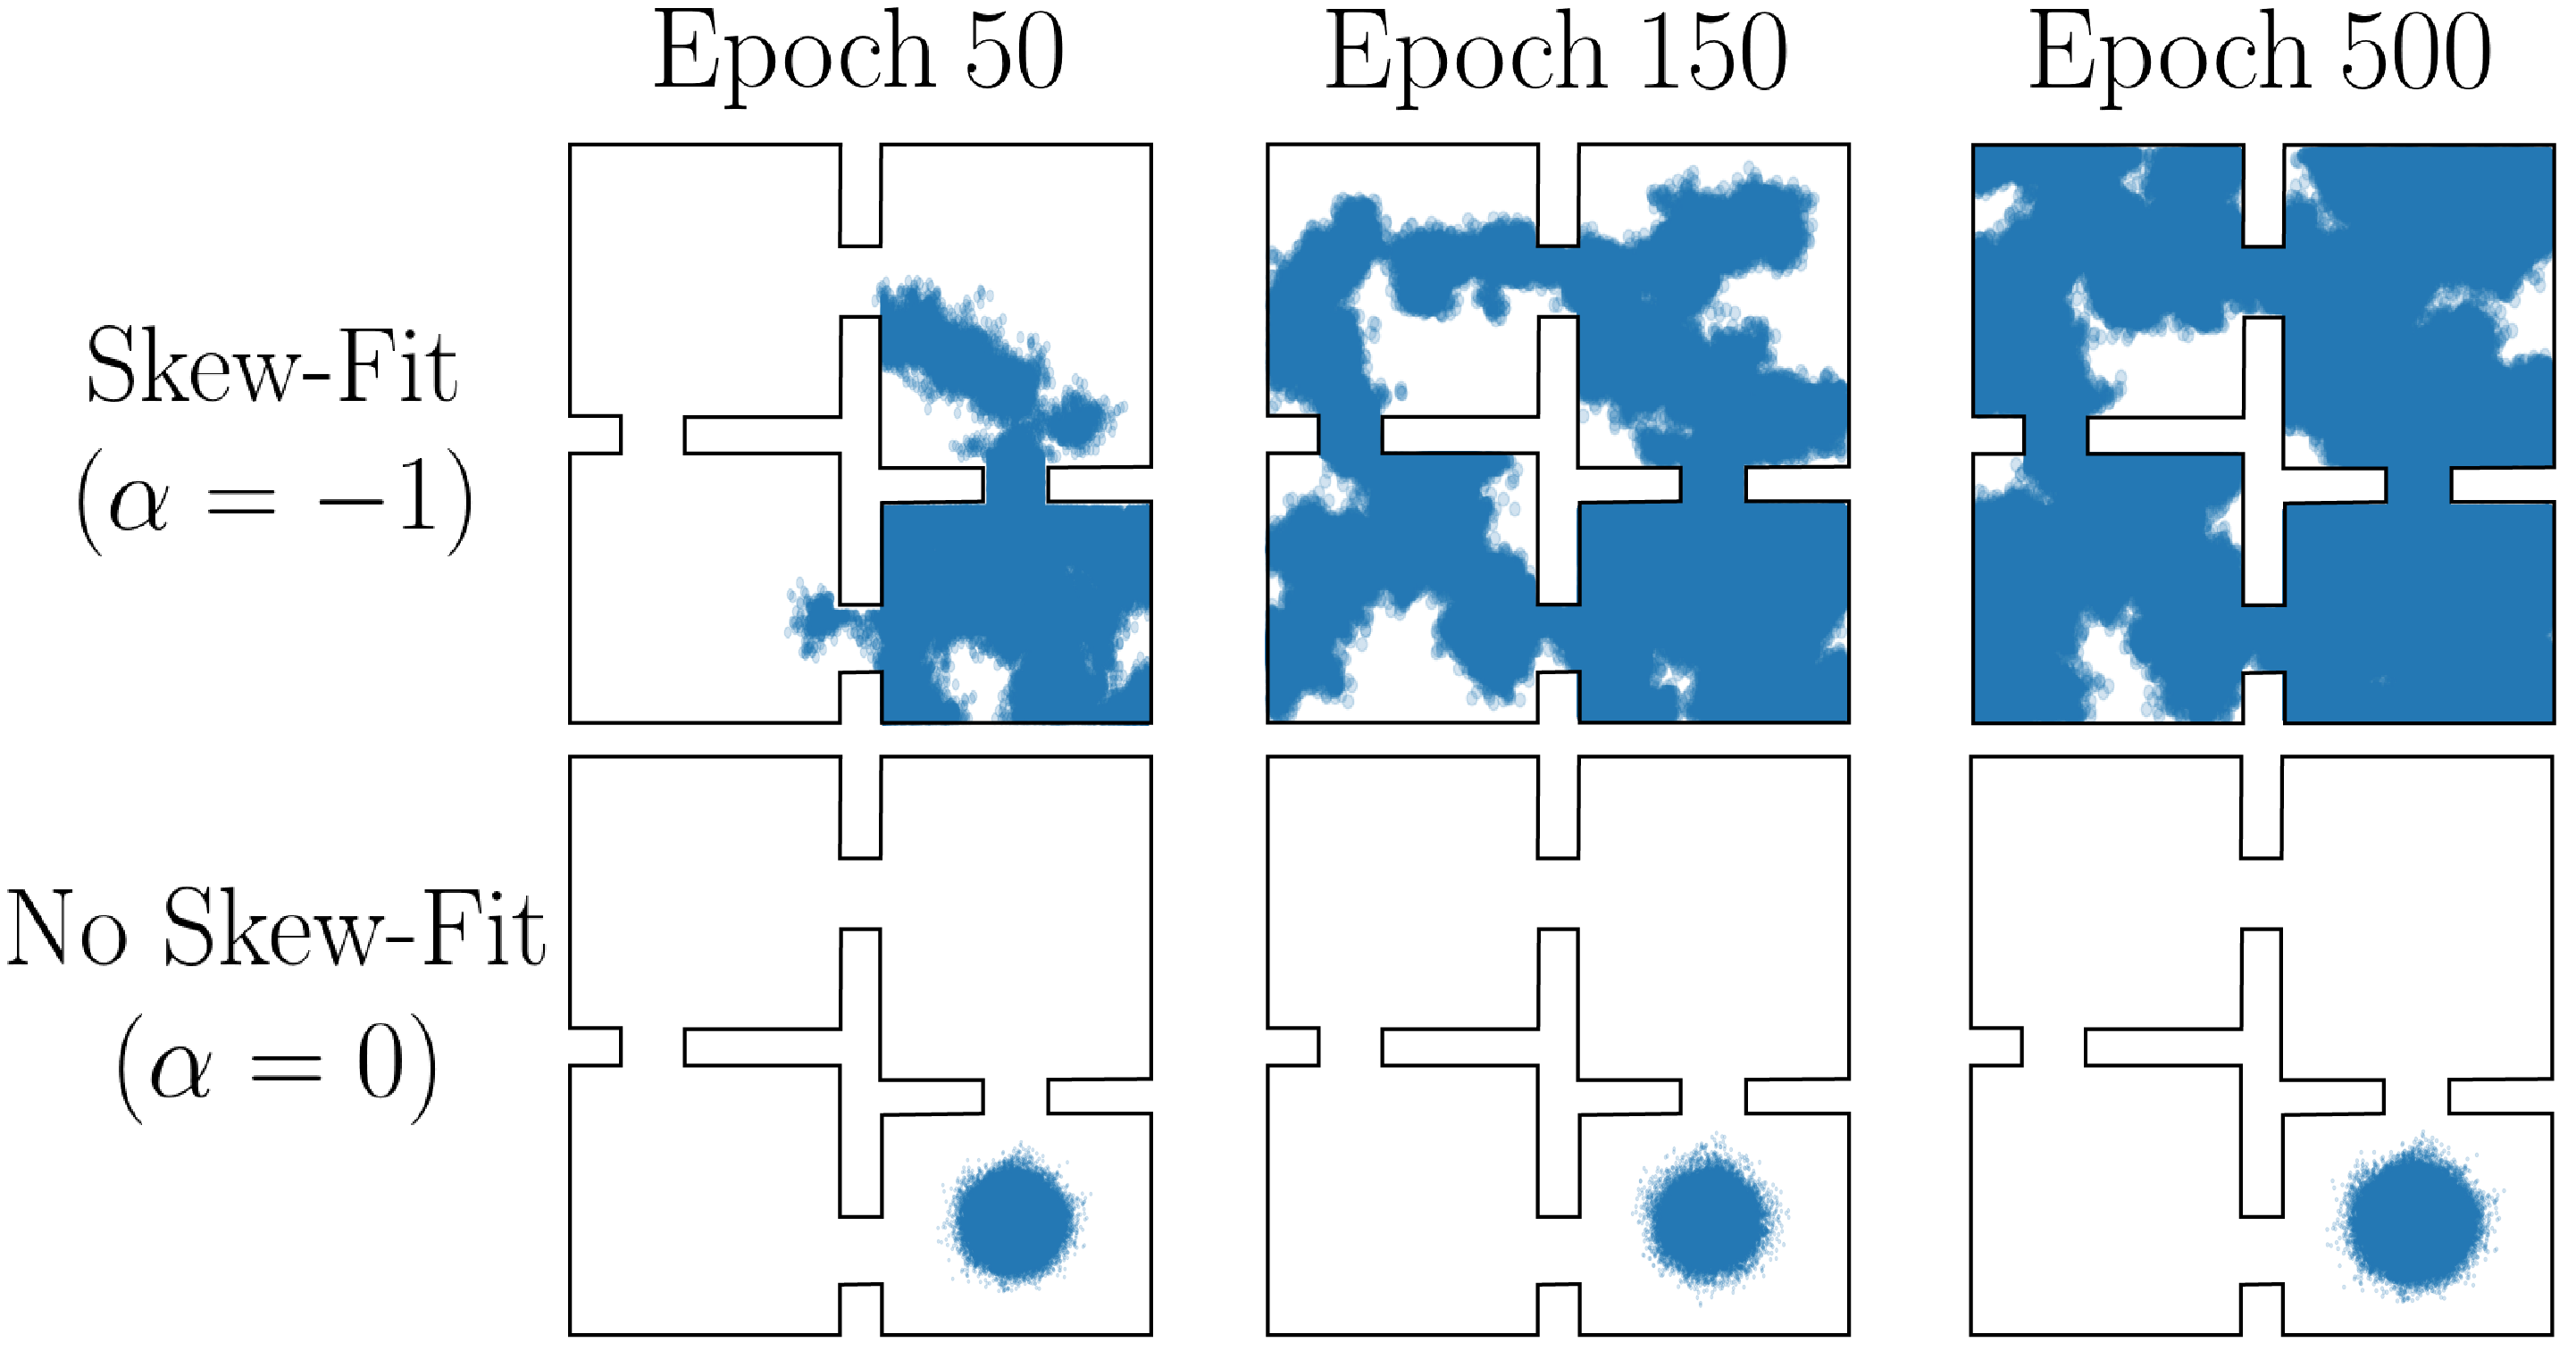
\includegraphics[width=.49\linewidth ]{skewfit/figures/entropy_figure-01.png}
    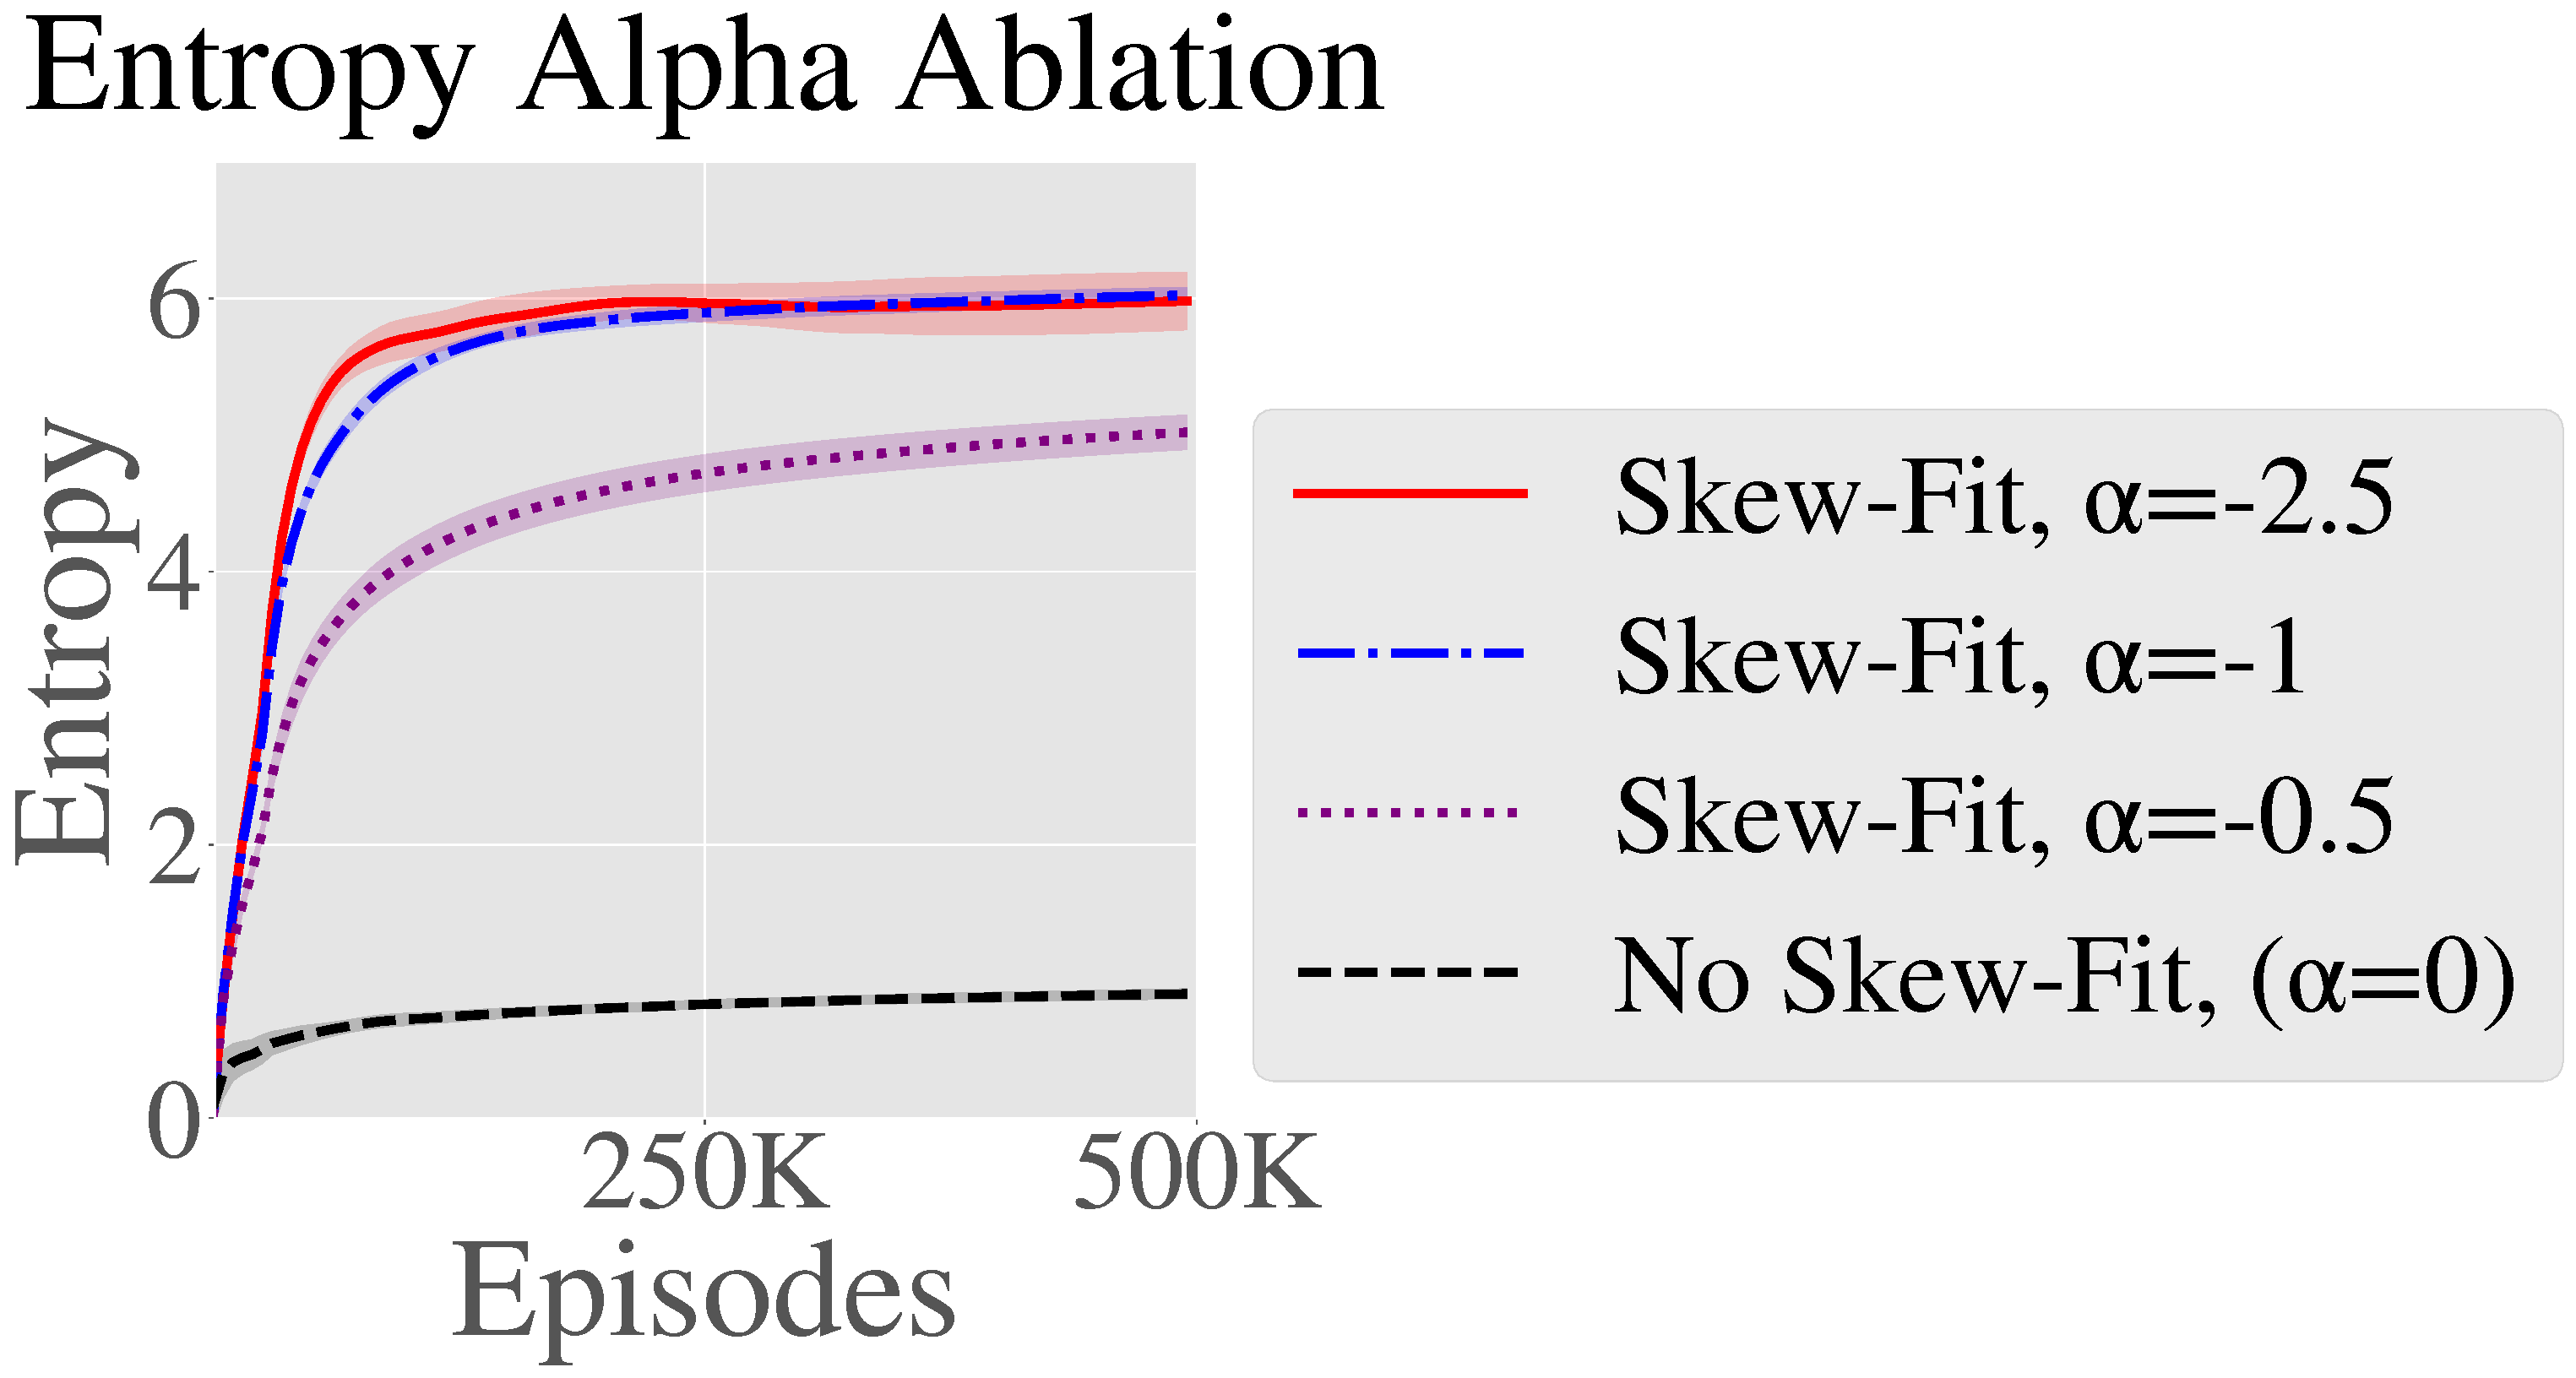
\includegraphics[width=.49\linewidth ]{skewfit/figures/plots/four_rooms_entropy}
    \caption{
    Illustrative example of \METHOD on a 2D navigation task. (Left) Visited state plot for \METHOD with $\alpha = -1$ and uniform sampling, which corresponds to $\alpha = 0$. (Right) The entropy of the goal distribution per iteration, mean and standard deviation for 9 seeds. Entropy is calculated via discretization onto an 11x11 grid. \METHOD steadily increases the state entropy, reaching full coverage over the state space.
    }
    \label{fig:2d-sl}
\end{figure}

\paragraph{Does \METHOD Maximize Entropy?}
To see the effects of \METHOD on goal distribution entropy in isolation of learning a goal-reaching policy, we study an idealized example where the policy is a near-perfect goal-reaching policy.
The environment consists of four rooms~\citep{sutton1999between}.
At the beginning of an episode, the agent begins in the bottom-right room and samples a goal from the goal distribution $\pgt$.
To simulate stochasticity of the policy and environment, we add a Gaussian noise with standard deviation of $0.06$ units to this goal, where the entire environment is $11 \times 11$ units.
The policy reaches the state that is closest to this noisy goal and inside the rooms, giving us a state sample $\st_n$ for training $\pgt$.
Due to the relatively small noise, the agent cannot rely on this stochasticity to explore the different rooms and must instead learn to set goals that are progressively farther and farther from the initial state.
We compare multiple values of $\alpha$, where $\alpha=0$ corresponds to not using \METHOD.
The $\beta$-VAE hyperparameters used to train $\pgt$ are given in \autoref{sec:2d-details}.
As seen in \Figref{fig:2d-sl}, sampling uniformly from previous experience ($\alpha = 0$) to set goals results in a policy that primarily sets goal near the initial state distribution.
In contrast, \METHOD results in quickly learning a high entropy, near-uniform distribution over the state space.

\begin{figure}[ht!]
    \centering
    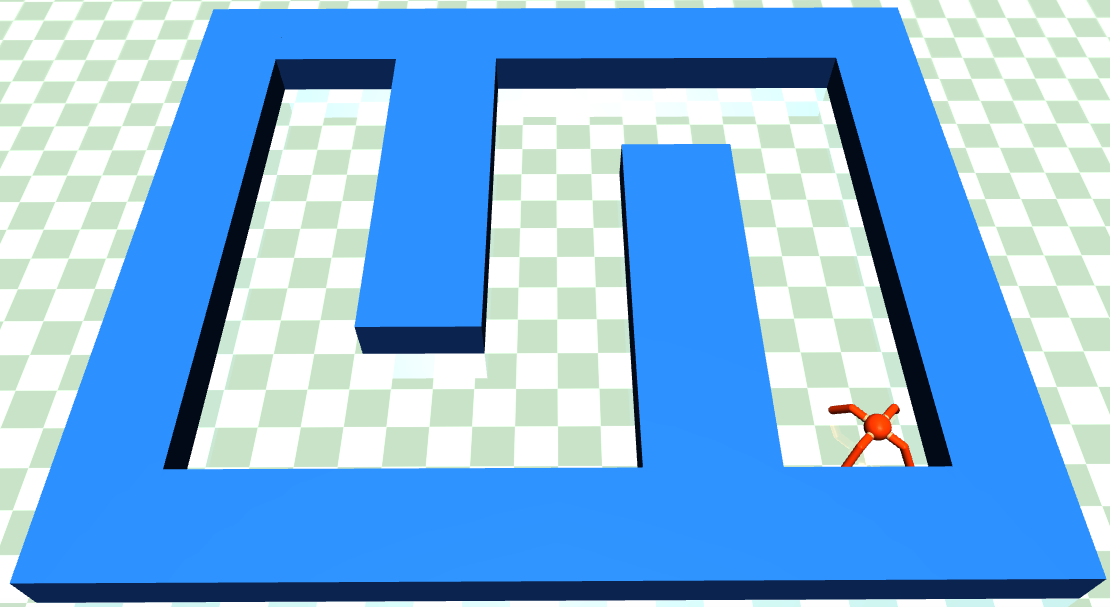
\includegraphics[width=0.32\linewidth]{skewfit/figures/ant_env_updated.png}
    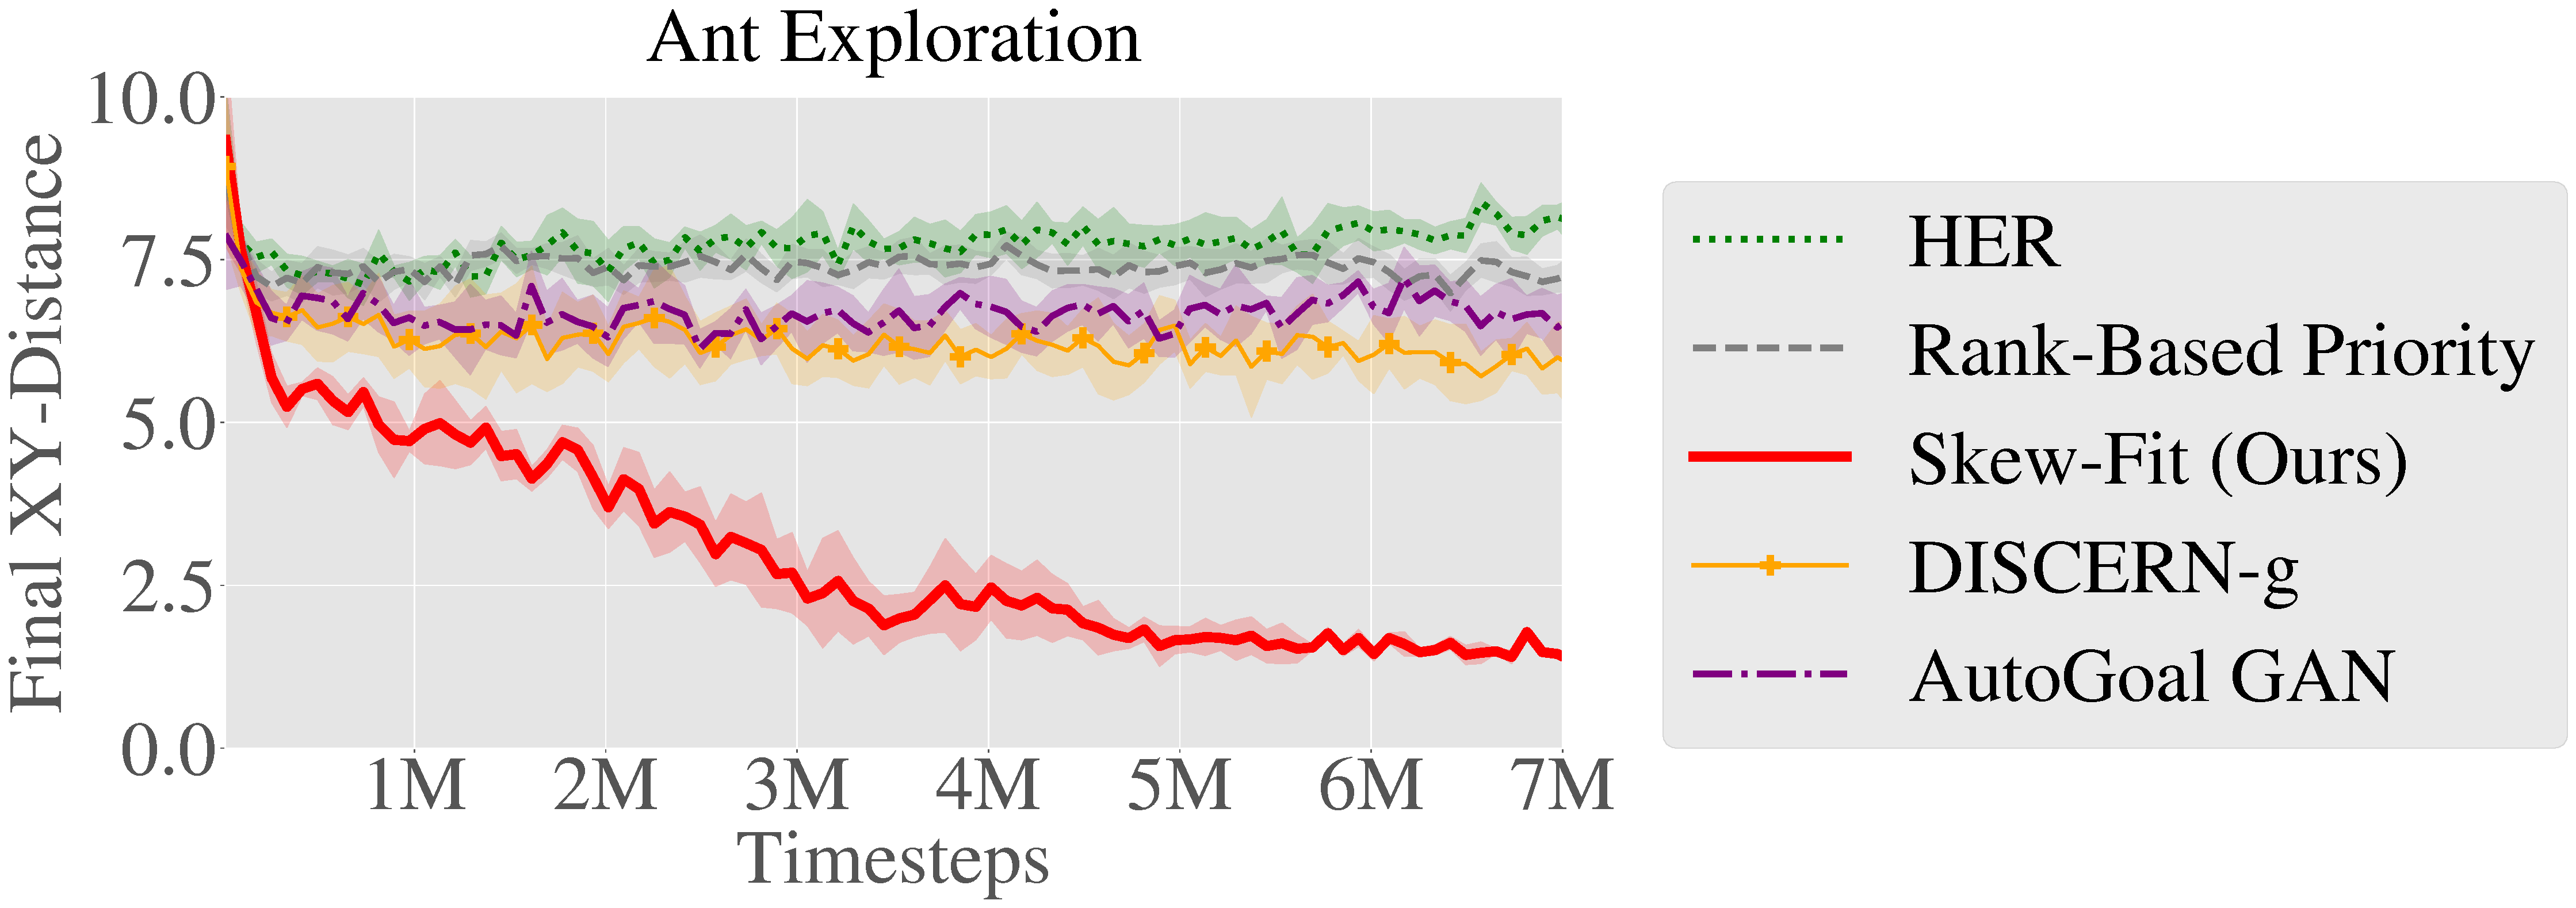
\includegraphics[width=0.65\linewidth]{skewfit/figures/plots/ant.pdf}
    \caption{
    (Left) Ant navigation environment.
    (Right) Evaluation on reaching target XY position.
    We show the mean and standard deviation of 6 seeds.
    \METHOD significantly outperforms prior methods on this exploration task.
    }
    \label{fig:antmaze}
\end{figure}

\paragraph{Exploration with \METHOD}
We next evaluate \METHOD while concurrently learning a goal-conditioned policy on a task with state inputs, which enables us study exploration performance independently of the challenges with image observations.
We evaluate on a task that requires training a simulated quadruped ``ant'' robot to navigate to different XY positions in a labyrinth,
as shown in \Figref{fig:antmaze}.
The reward is the negative distance to the goal XY-position, and additional environment details are provided in \autoref{sec:environment-details}.
This task presents a challenge for goal-directed exploration:
the set of valid goals is unknown due to the walls, and
random actions do not result in exploring locations far from the start.
Thus, \METHOD must set goals that meaningfully explore the space while simultaneously learning to reach those goals.

We use this domain to compare \METHOD to a number of existing goal-sampling methods.
We compare to the relabeling scheme described in the hindsight experience replay (labeled \textbf{HER}).
We compare to curiosity-driven prioritization (\textbf{Ranked-Based Priority})~\citep{zhao2019maximum}, a variant of HER that samples goals for relabeling based on their ranked likelihoods.
\citet{held2018goalgan} samples goals from a GAN based on the difficulty of reaching the goal.
We compare against this method by replacing $\pg$ with the GAN and label it \textbf{AutoGoal GAN}.
We also compare to the non-parametric goal proposal mechanism proposed by \cite{wardefarley2018discern}, which we label \textbf{DISCERN-g}.
Lastly, to demonstrate the difficulty of the exploration challenge in these domains, we compare to \textbf{\#-Exploration}~\citep{tang2017hashtag}, an exploration method that assigns bonus rewards based on the novelty of new states.
We train the goal-conditioned policy for each method using soft actor critic (SAC)~\citep{haarnoja2018sacapp}.
Implementation details of SAC and the prior works are given in  \autoref{sec:prior-work-implementation}.

We see in \Figref{fig:antmaze} that \METHOD is the only method that makes significant progress on this challenging labyrinth locomotion task.
The prior methods on goal-sampling primarily set goals close to the start location, while the extrinsic exploration reward in \#-Exploration dominated the goal-reaching reward.
These results demonstrate that \METHOD accelerates exploration by setting diverse goals in tasks with unknown goal spaces.


\paragraph{Vision-Based Continuous Control Tasks}
\begin{figure}[ht!]
    \centering
    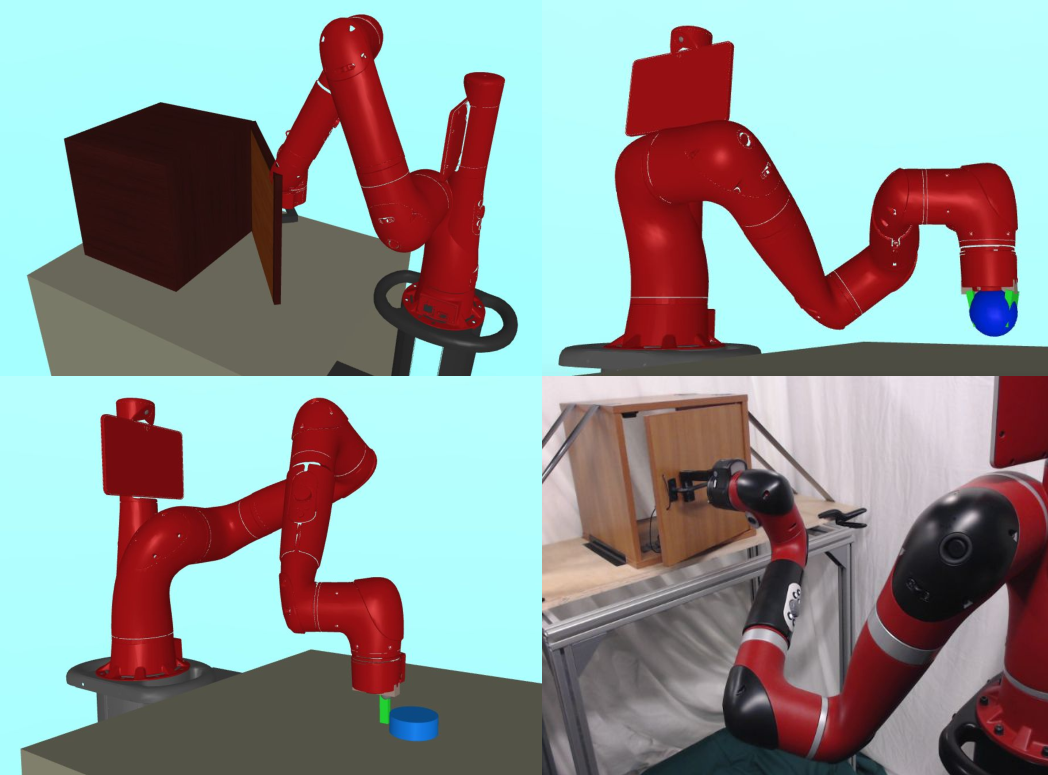
\includegraphics[width=0.9\linewidth]{skewfit/figures/env_display.pdf}
    \caption{We evaluate on these continuous control tasks, from left to right:
    \textit{Visual Door}, a door opening task;
    \textit{Visual Pickup}, a picking task;
    \textit{Visual Pusher}, a pushing task;
    and \textit{Real World Visual Door}, a real world door opening task. All tasks are solved from images and without any task-specific reward. See Appendix \ref{sec:environment-details} for details.}
    \label{fig:env-pics}
\end{figure}

We now evaluate \METHOD on a variety of image-based continuous control tasks, where the policy must control a robot arm using only image observations, there is no state-based or task-specific reward, and \METHOD must directly set image goals.
We test our method on three different image-based simulated continuous control tasks released by the authors of RIG~\citep{nair2018rig}: \textit{Visual Door}, \textit{Visual Pusher}, and \textit{Visual Pickup}.
These environments contain a robot that can open a door, push a puck, and lift up a ball to different configurations, respectively.
To our knowledge, these are the only goal-conditioned, vision-based continuous control environments that are publicly available and experimentally evaluated in prior work, making them a good point of comparison.
See \autoref{fig:env-pics} for visuals and \autoref{sec:implementation-details} for environment details.
The policies are trained in a completely unsupervised manner, without access to any prior information about the image-space or any pre-defined goal-sampling distribution.
To evaluate their performance, we sample goal images from a uniform distribution over valid states and report the agent's final distance to the corresponding simulator states (e.g., distance of the object to the target object location), but the agent never has access to this true uniform distribution nor the ground-truth state information during training.
While this evaluation method is only practical in simulation, it provides us with a quantitative measure of a policy's ability to reach a broad coverage of goals in a vision-based setting.

We compare \METHOD to a number of existing methods on this domain.
First, we compare to the methods described in the previous experiment (HER, Rank-Based Priority, \#-Exploration, Autogoal GAN, and \mbox{DISCERN-g}).
These methods that we compare to were developed in non-vision, state-based environments.
To ensure a fair comparison across methods, we combine these prior methods with a policy trained using RIG.
We additionally compare to \citet{hazan2019provably}, an exploration method that assigns bonus rewards based on the likelihood of a state (labeled \textbf{Hazan et al.}).
Next, we compare to \textbf{RIG} without \METHOD.
Lastly, we compare to \textbf{DISCERN}~\citep{wardefarley2018discern}, a vision-based method which uses a non-parametric clustering approach to sample goals and an image discriminator to compute rewards.

\begin{figure}[ht!]
    \centering
     \begin{subfigure}[t]{.49\linewidth}
    \centering
        % 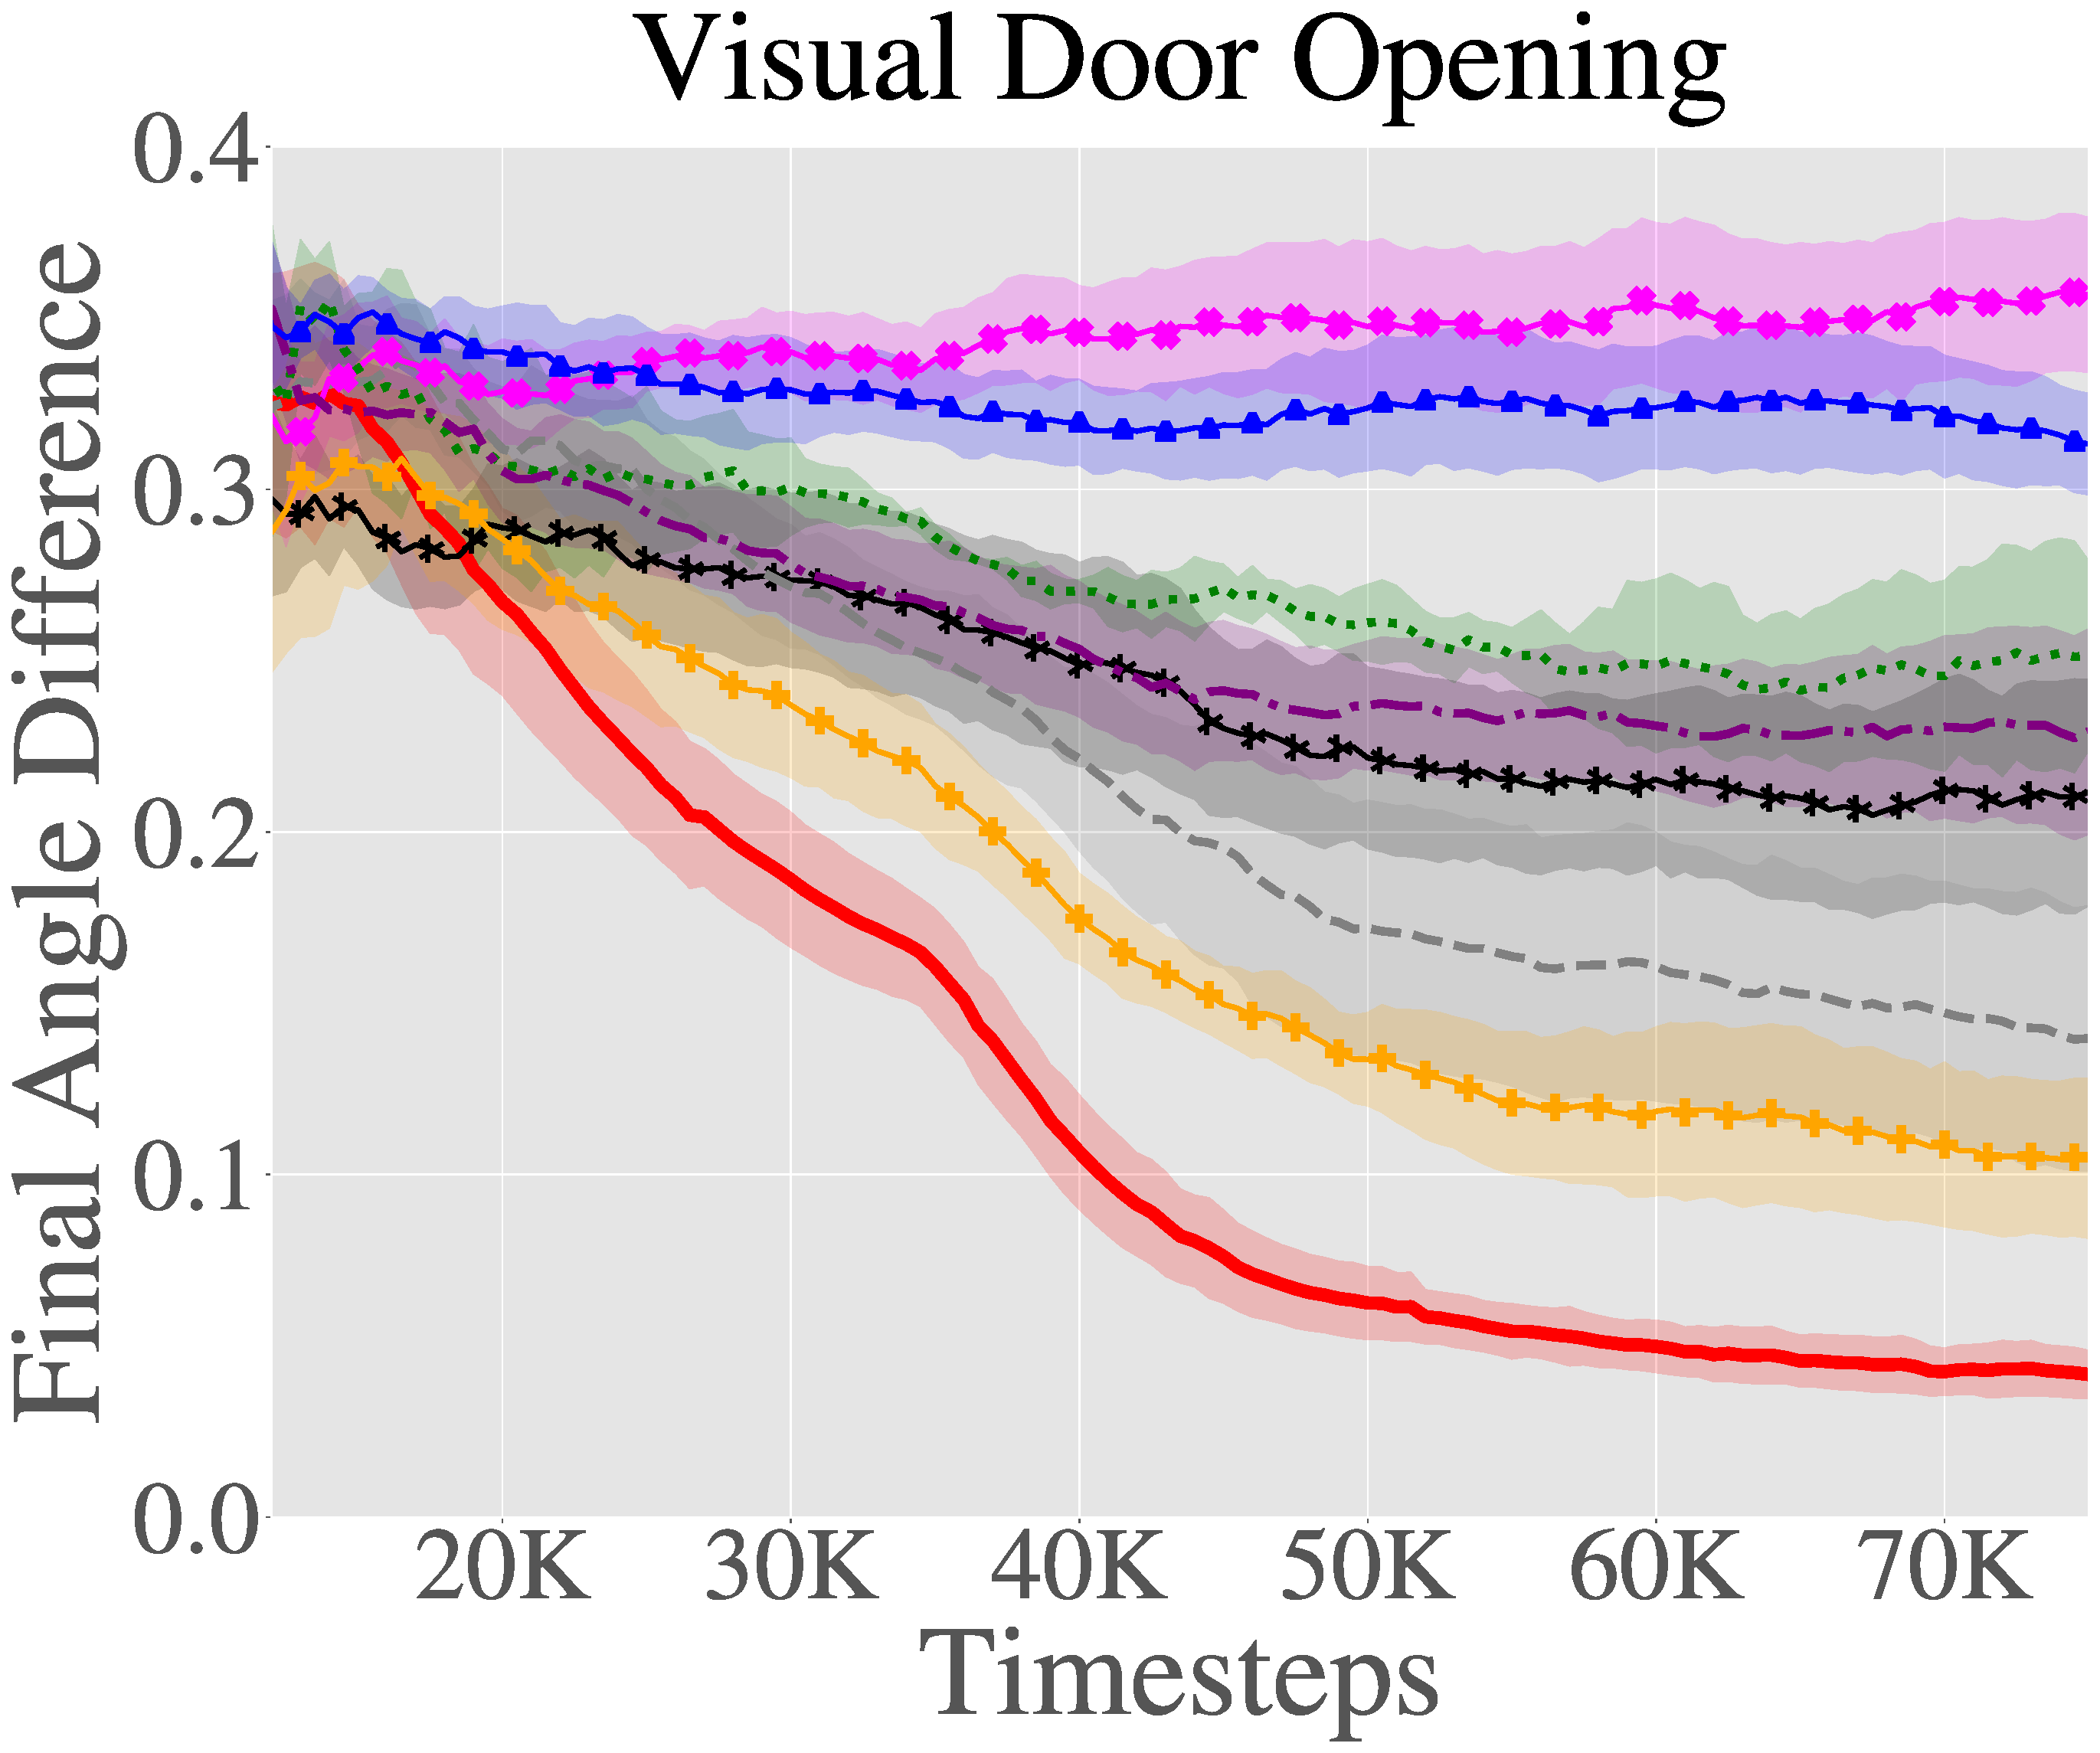
\includegraphics[width=\linewidth]{skewfit/figures/plots/main_sim_fig/door_big.pdf}
          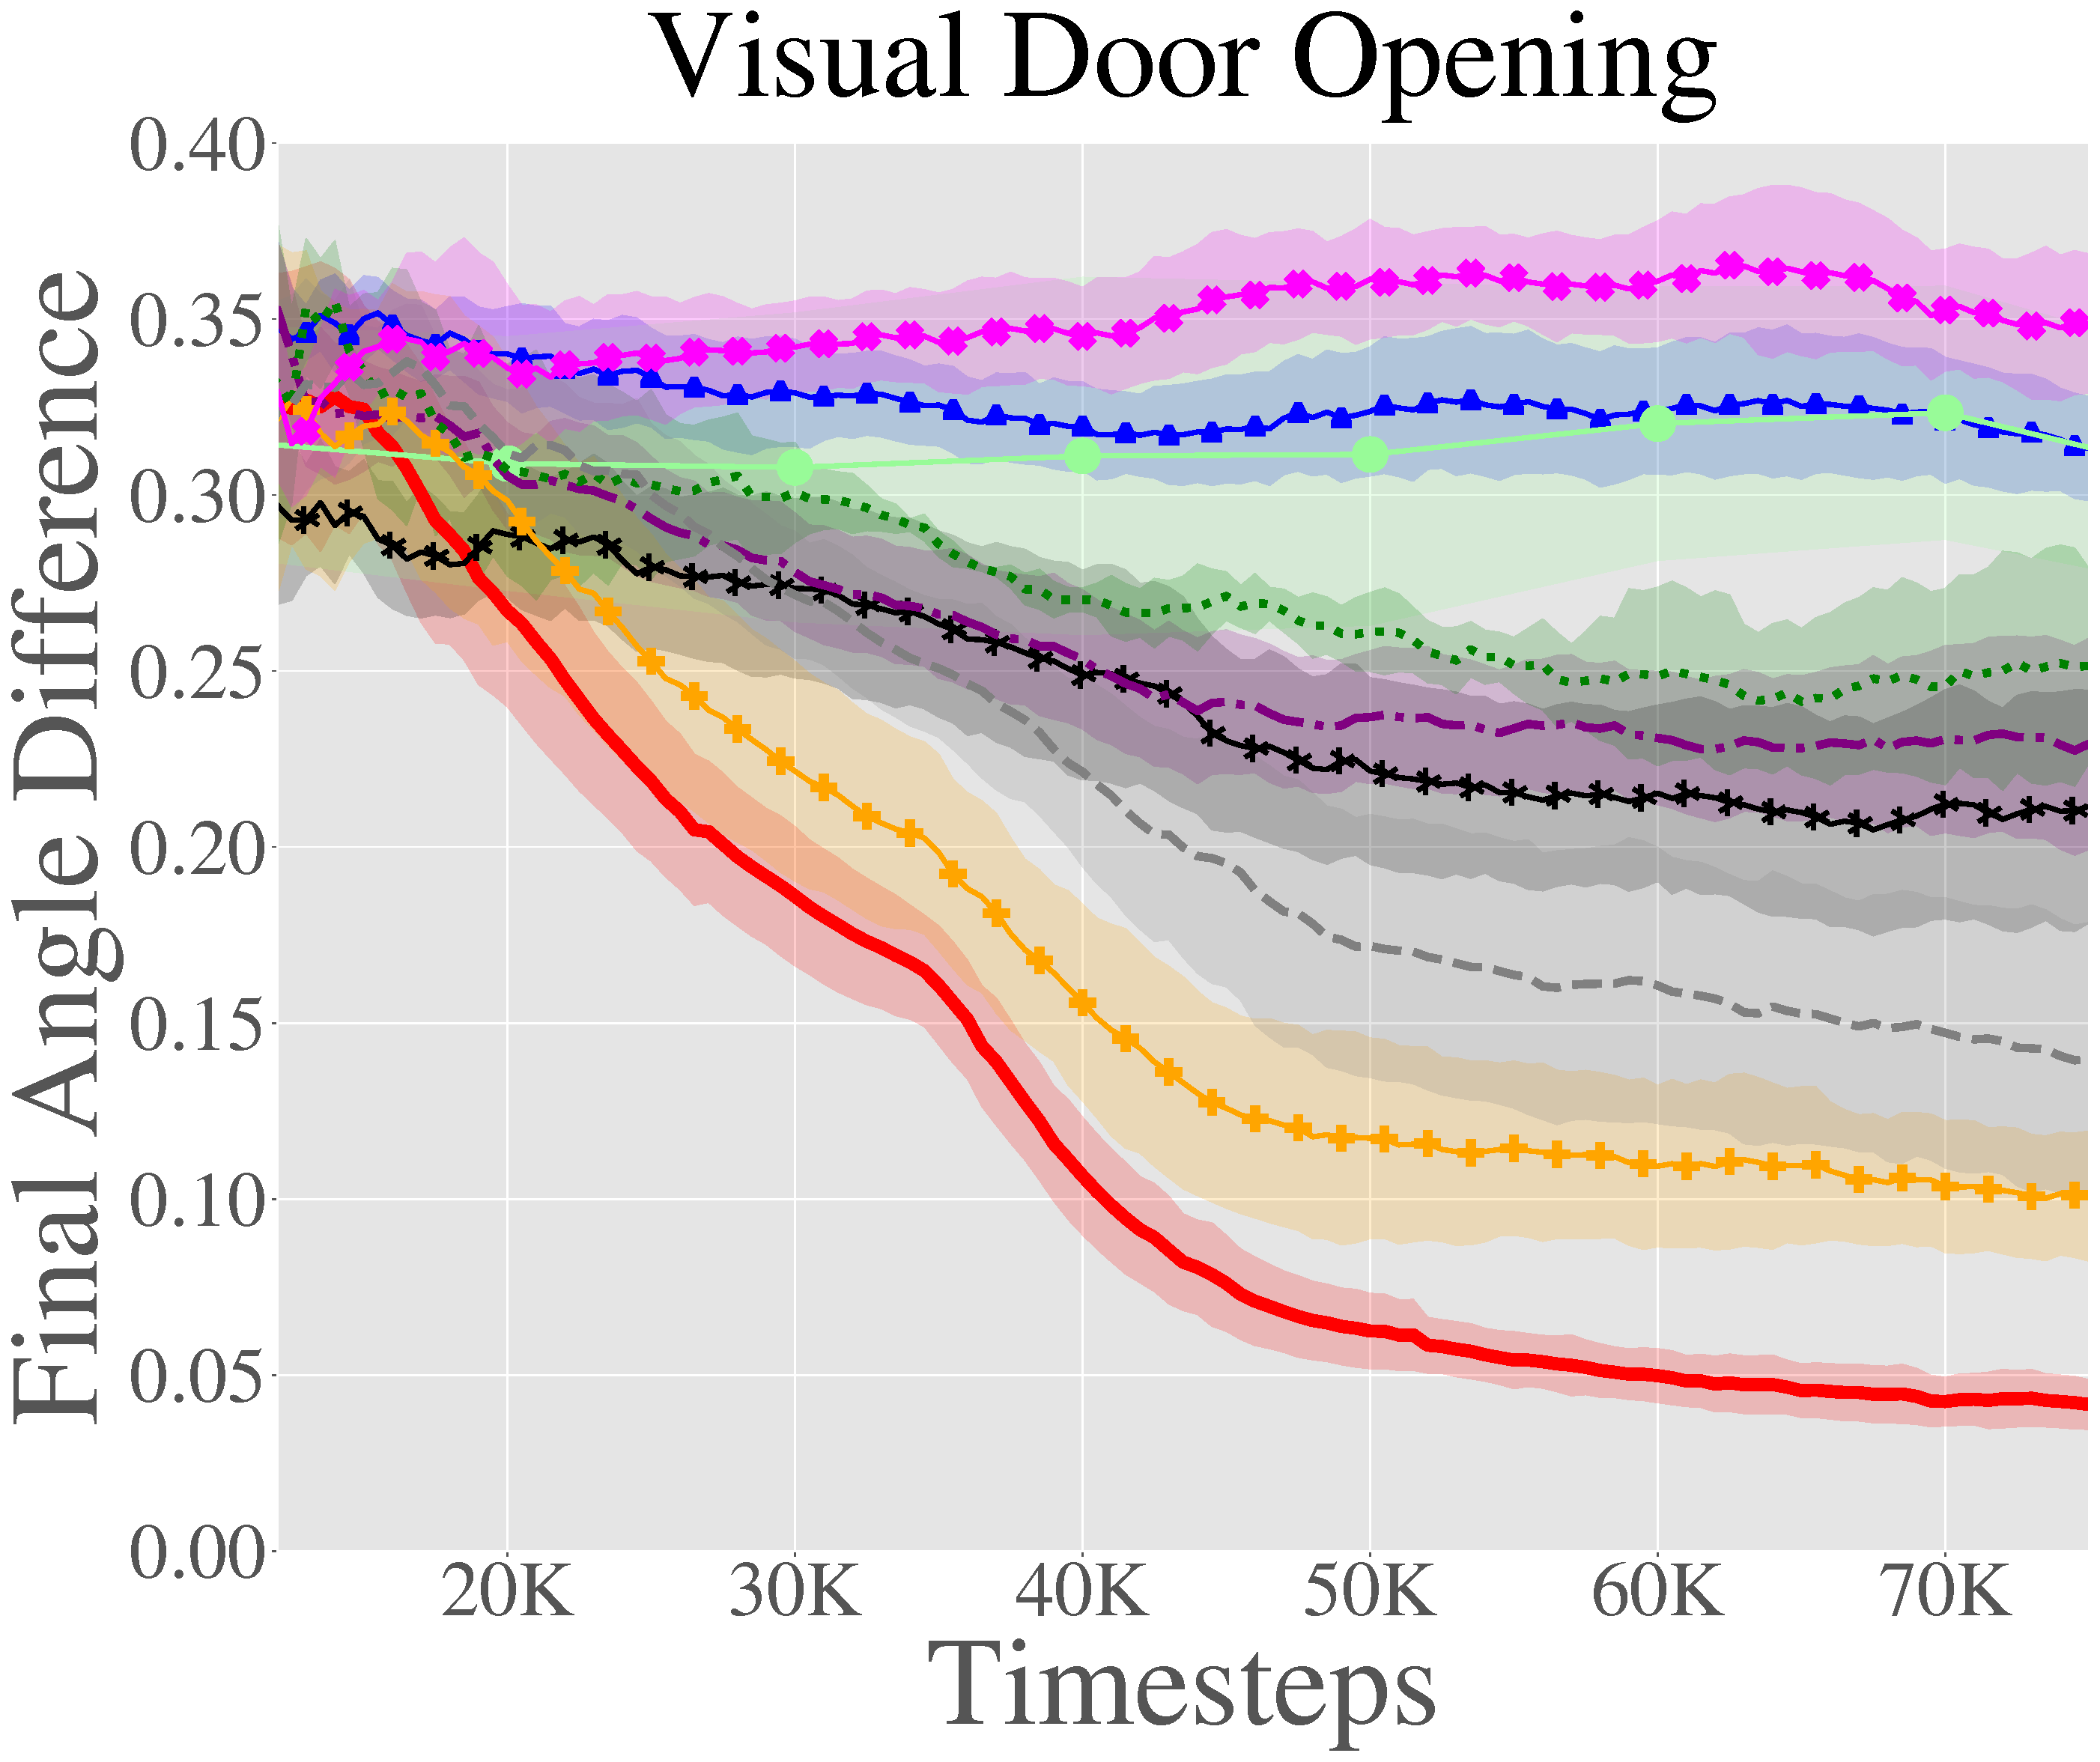
\includegraphics[width=\linewidth]{skewfit/figures/plots/main_sawyer_fig_with_hazan/door.pdf}
  \end{subfigure}
  \hfill
  \begin{subfigure}[t]{.49\linewidth}
    \centering
        % 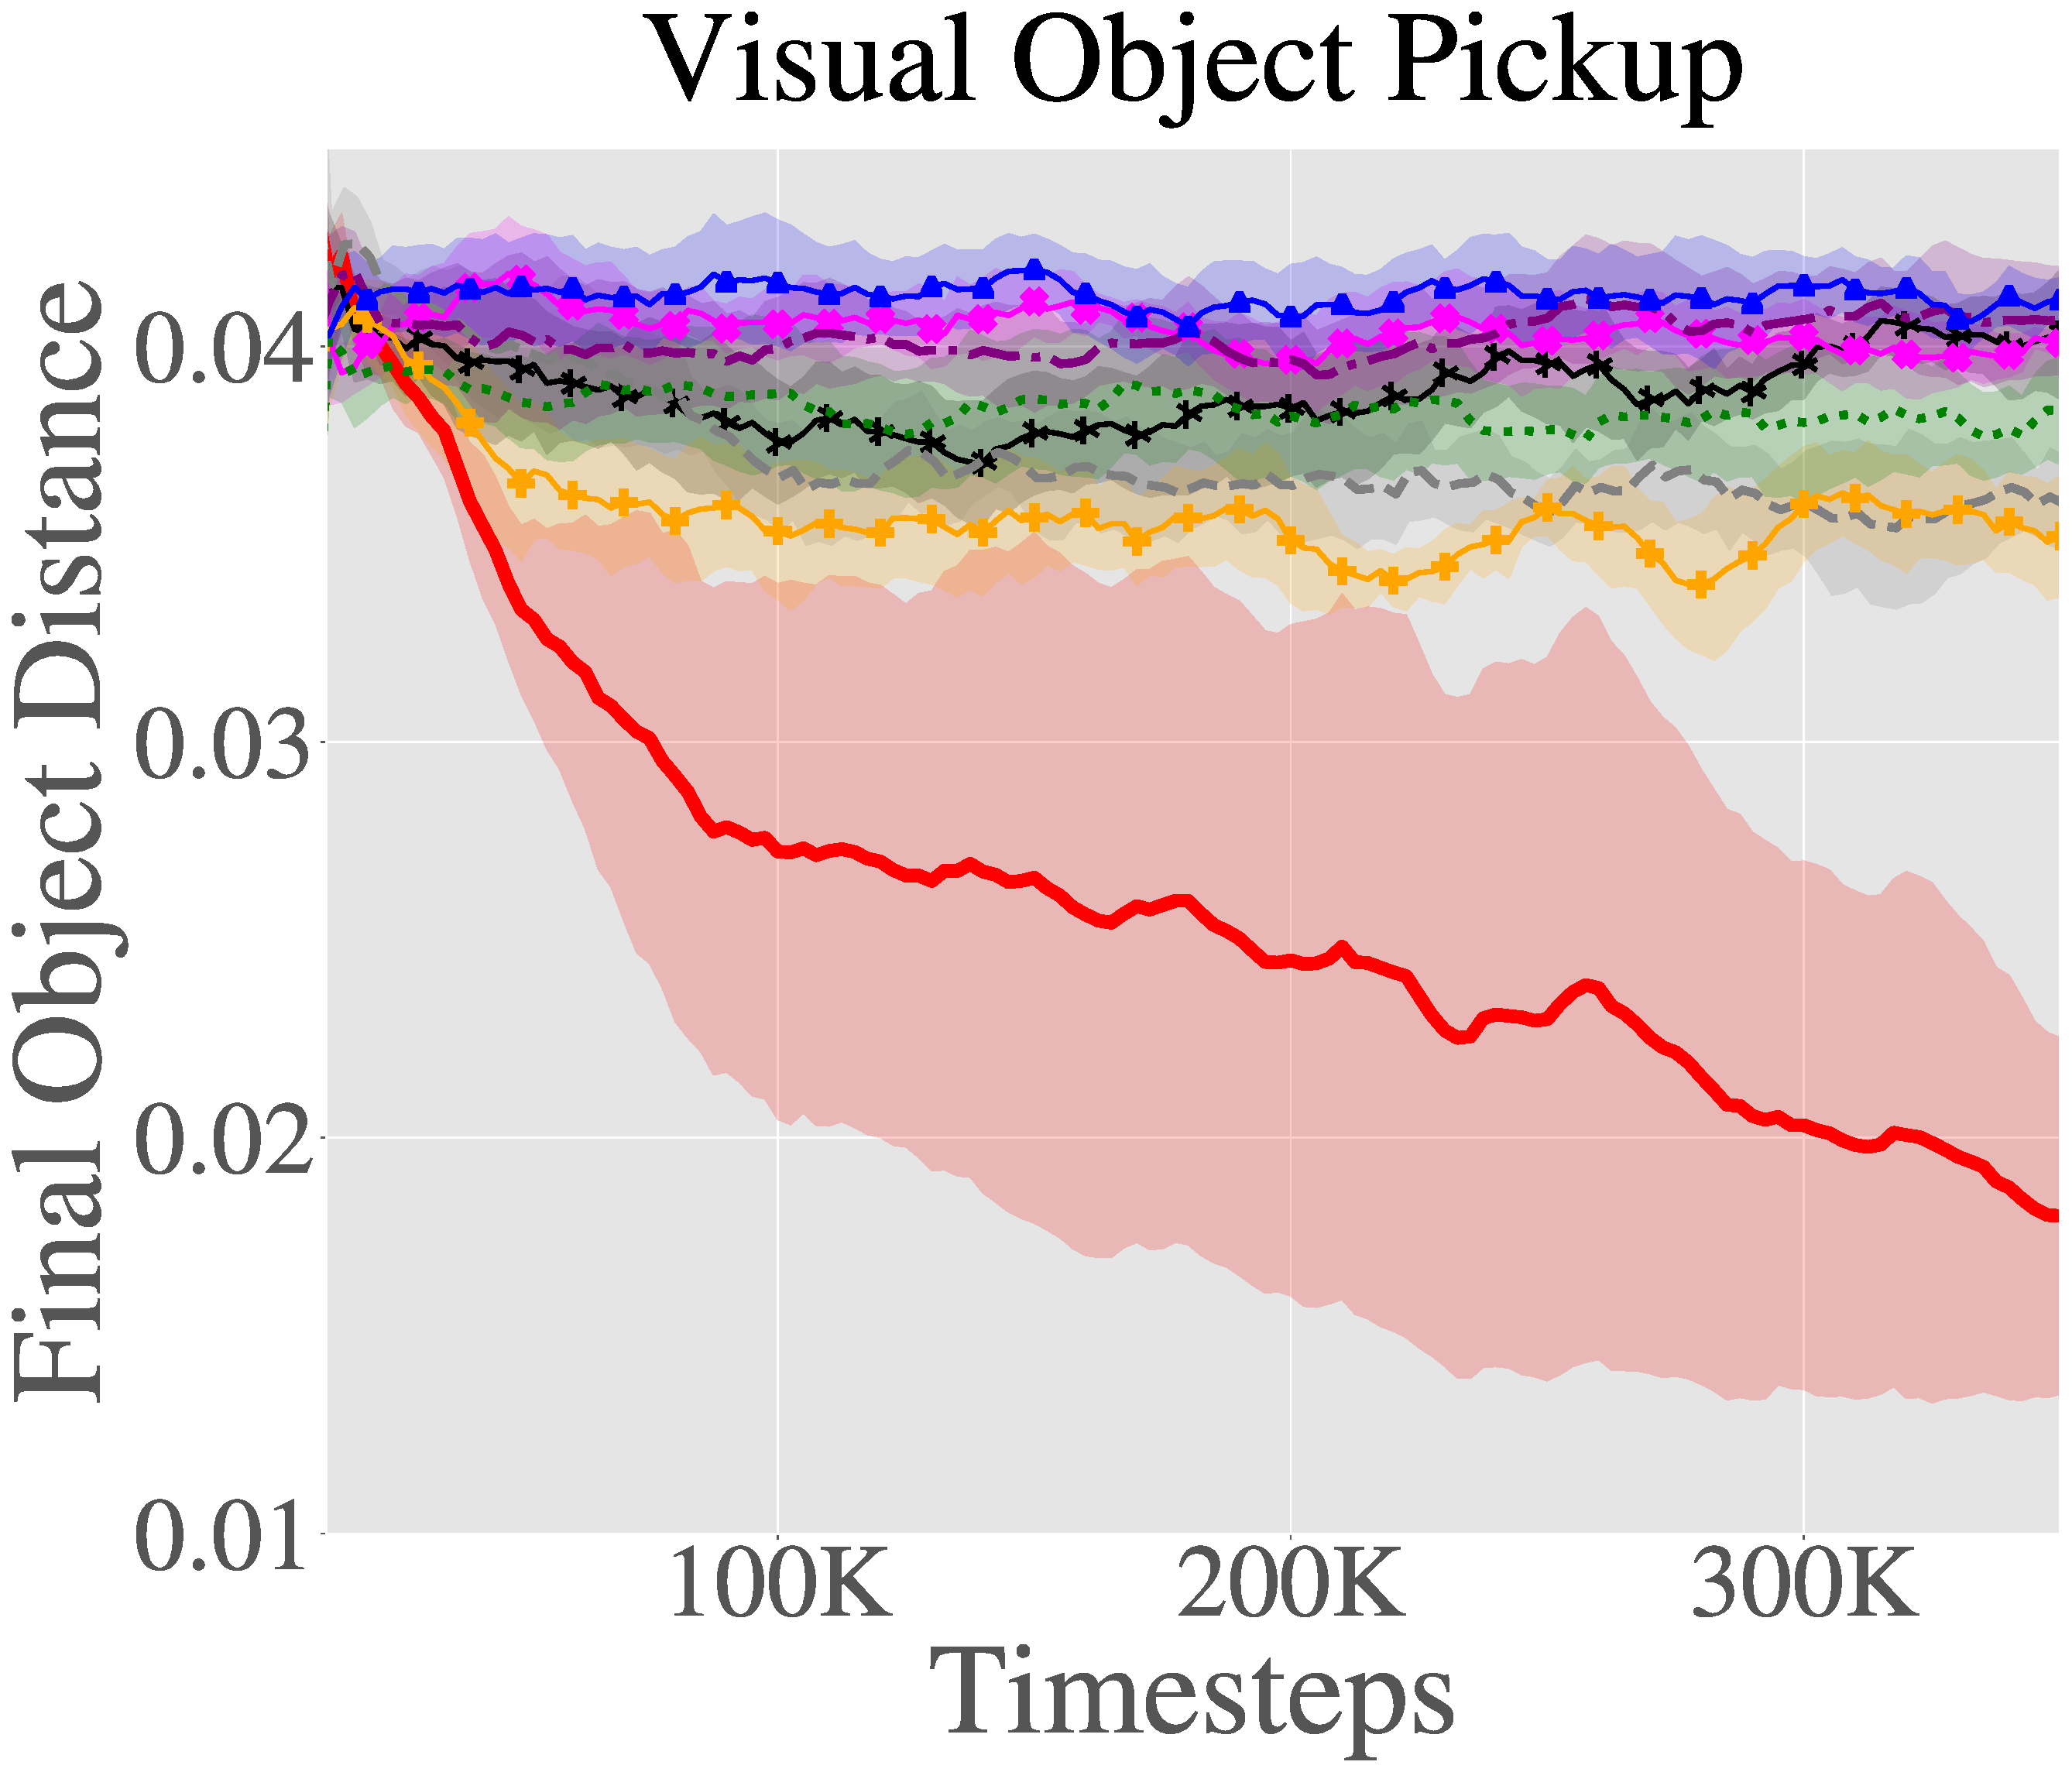
\includegraphics[width=\linewidth]{skewfit/figures/plots/main_sim_fig/pickup_big.pdf}
          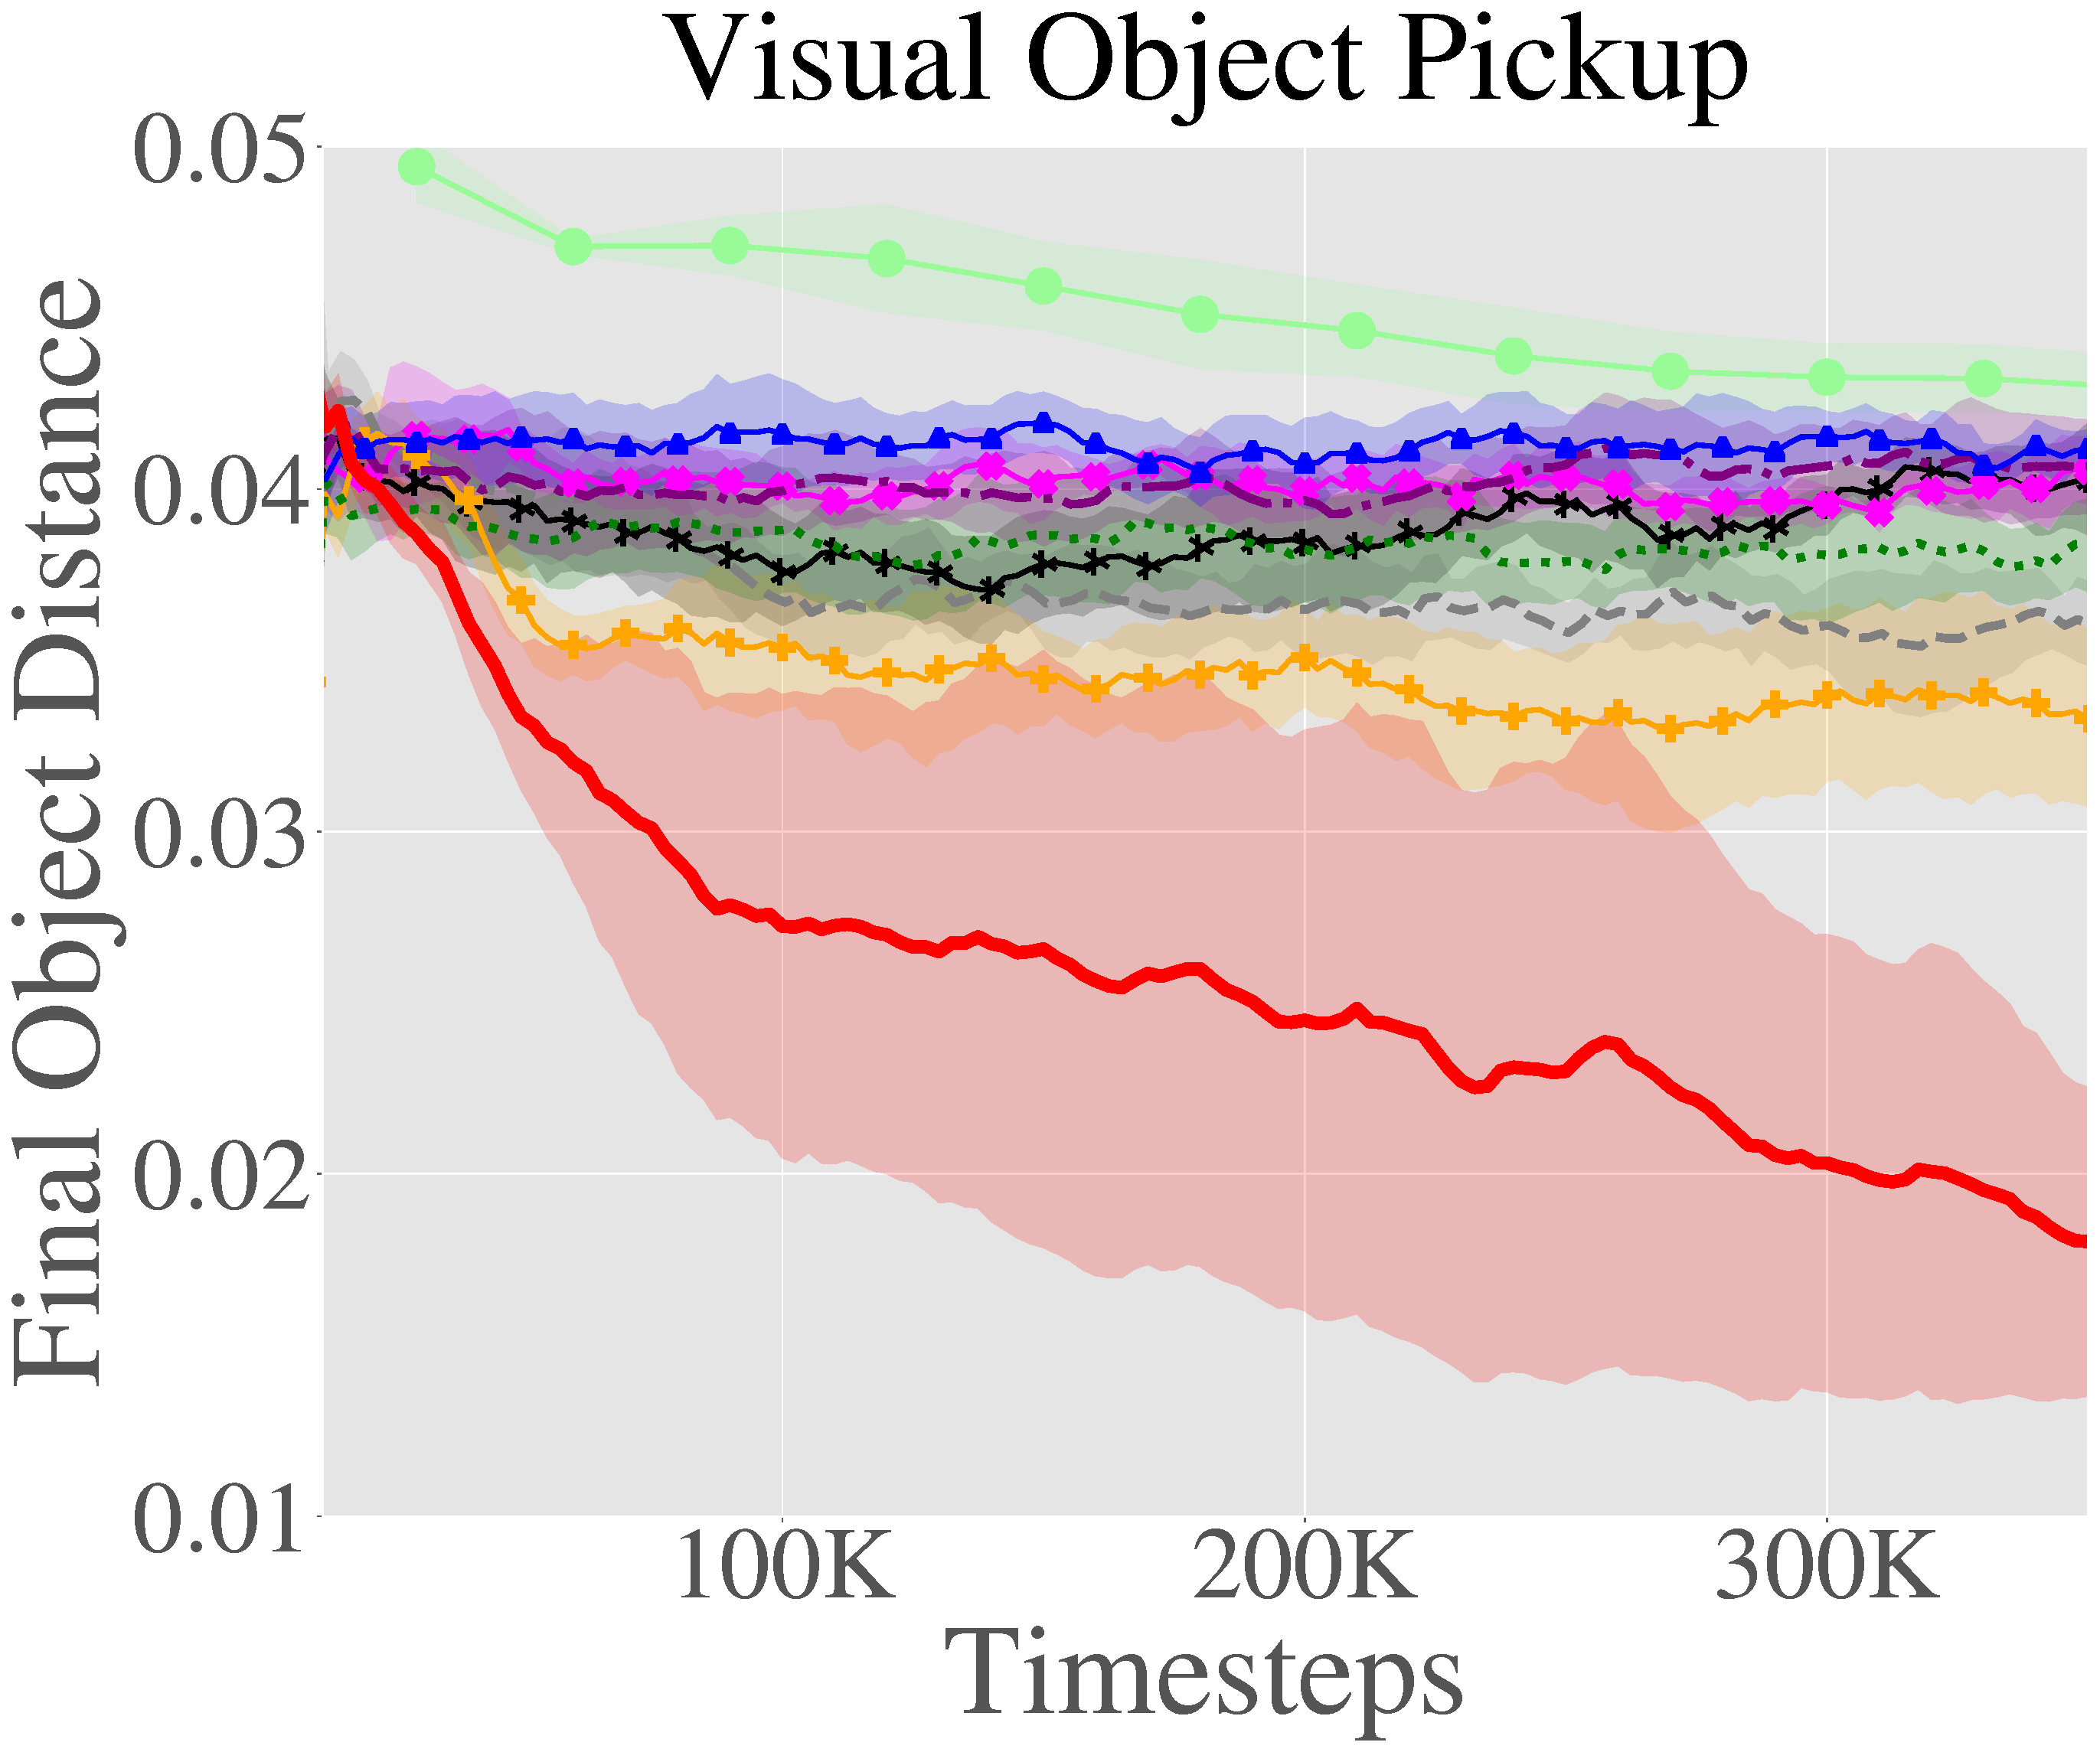
\includegraphics[width=\linewidth]{skewfit/figures/plots/main_sawyer_fig_with_hazan/pickup.pdf}
  \end{subfigure}

  \medskip

  \begin{subfigure}[t]{.49\linewidth}
    \centering
        %   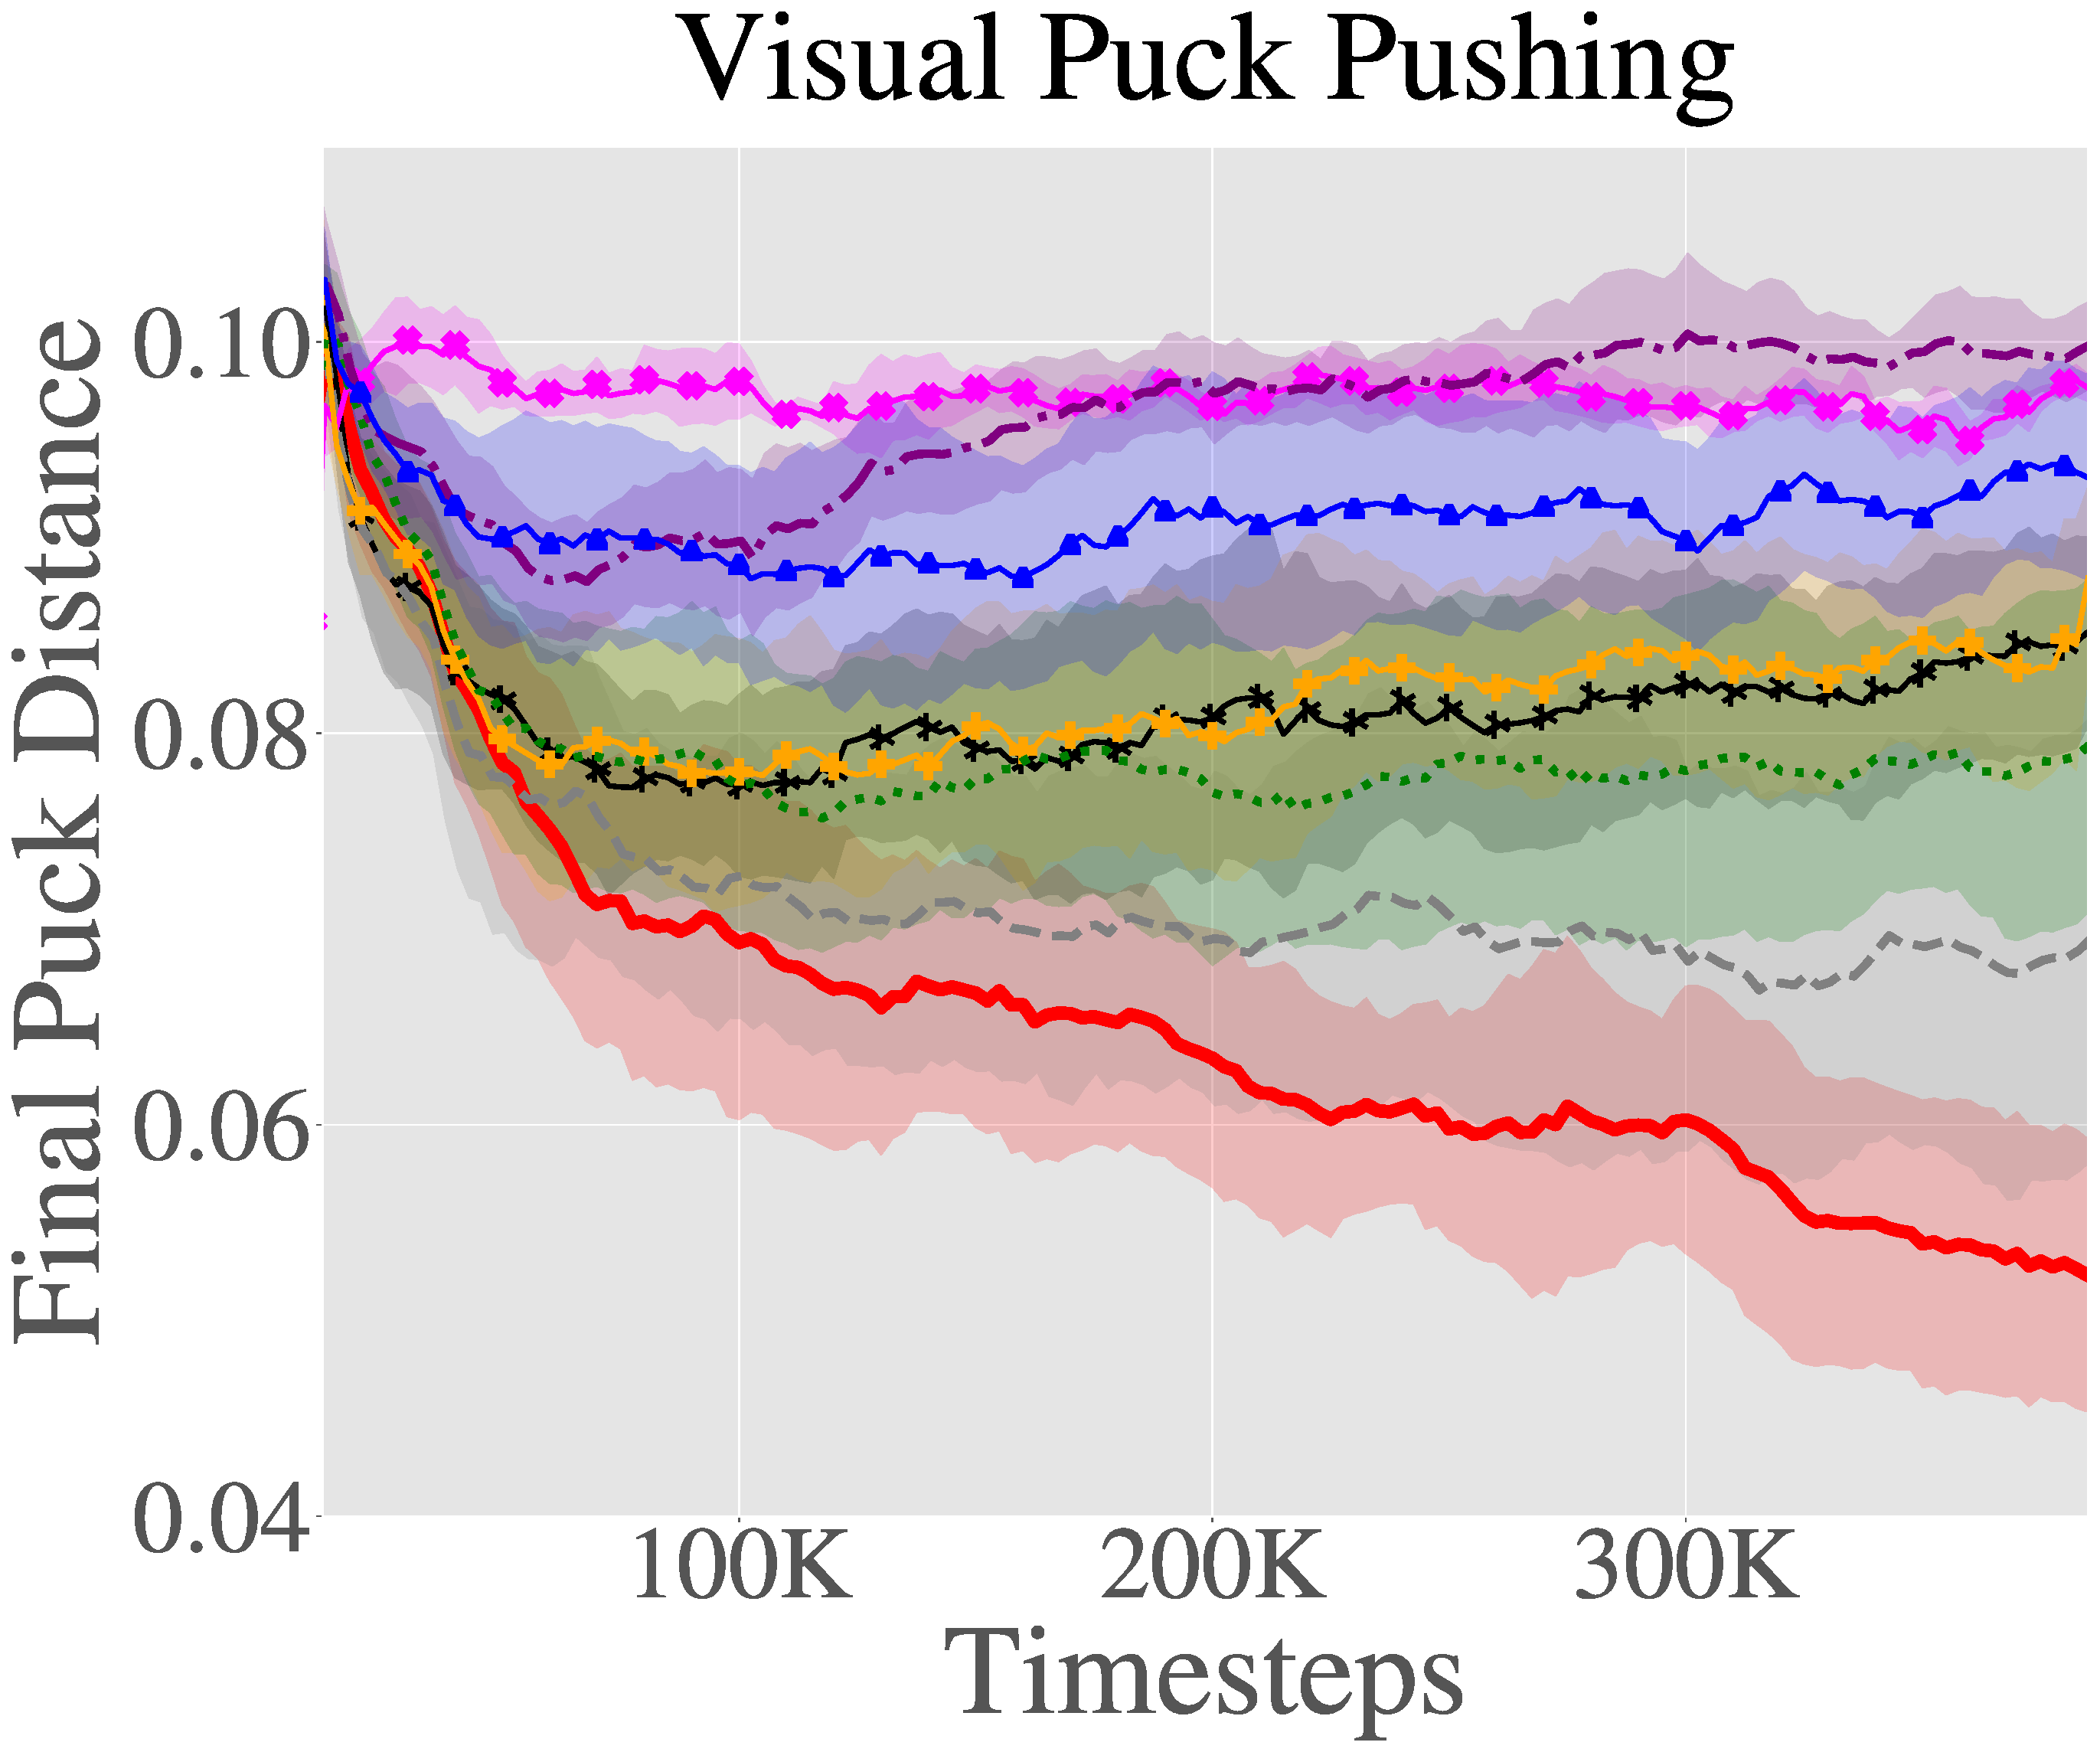
\includegraphics[width=\linewidth]{skewfit/figures/plots/main_sim_fig/pusher_big.pdf}
          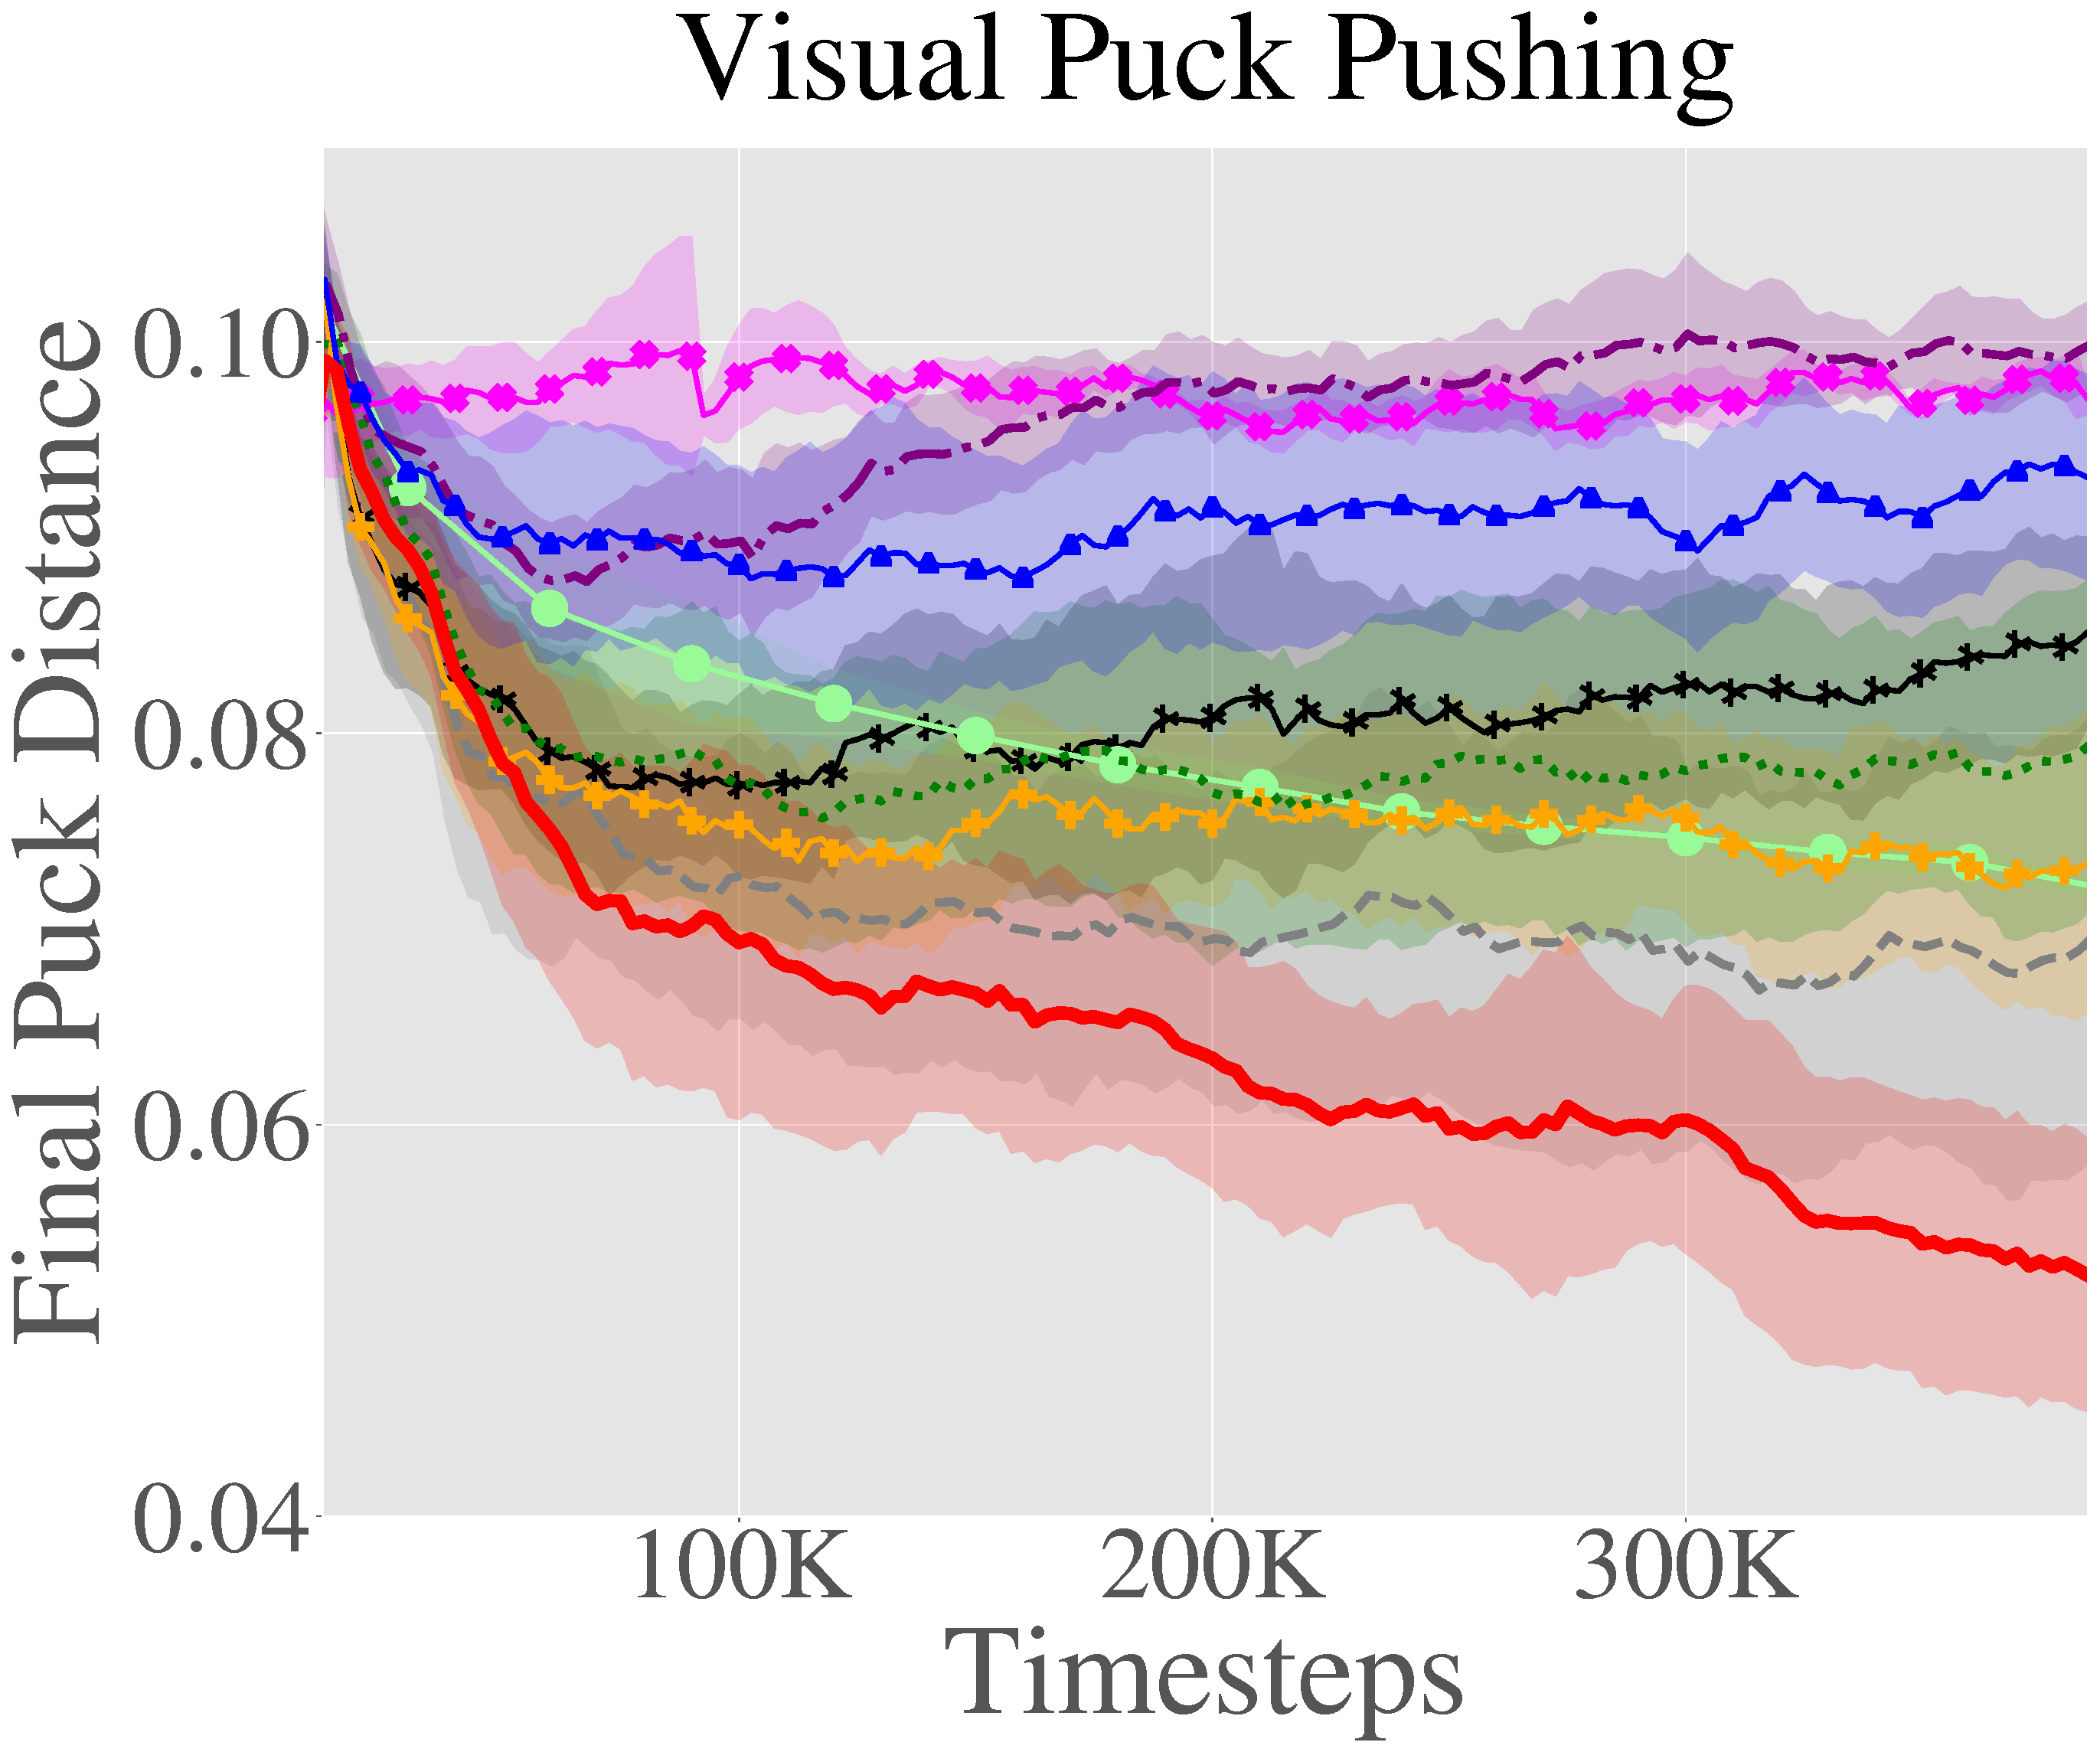
\includegraphics[width=\linewidth]{skewfit/figures/plots/main_sawyer_fig_with_hazan/pusher.pdf}
  \end{subfigure}
  \hfill
  \begin{subfigure}[t]{.48\linewidth}
    \centering
    % \hspace{0.165in}
    \raisebox{0.16in}{
        % 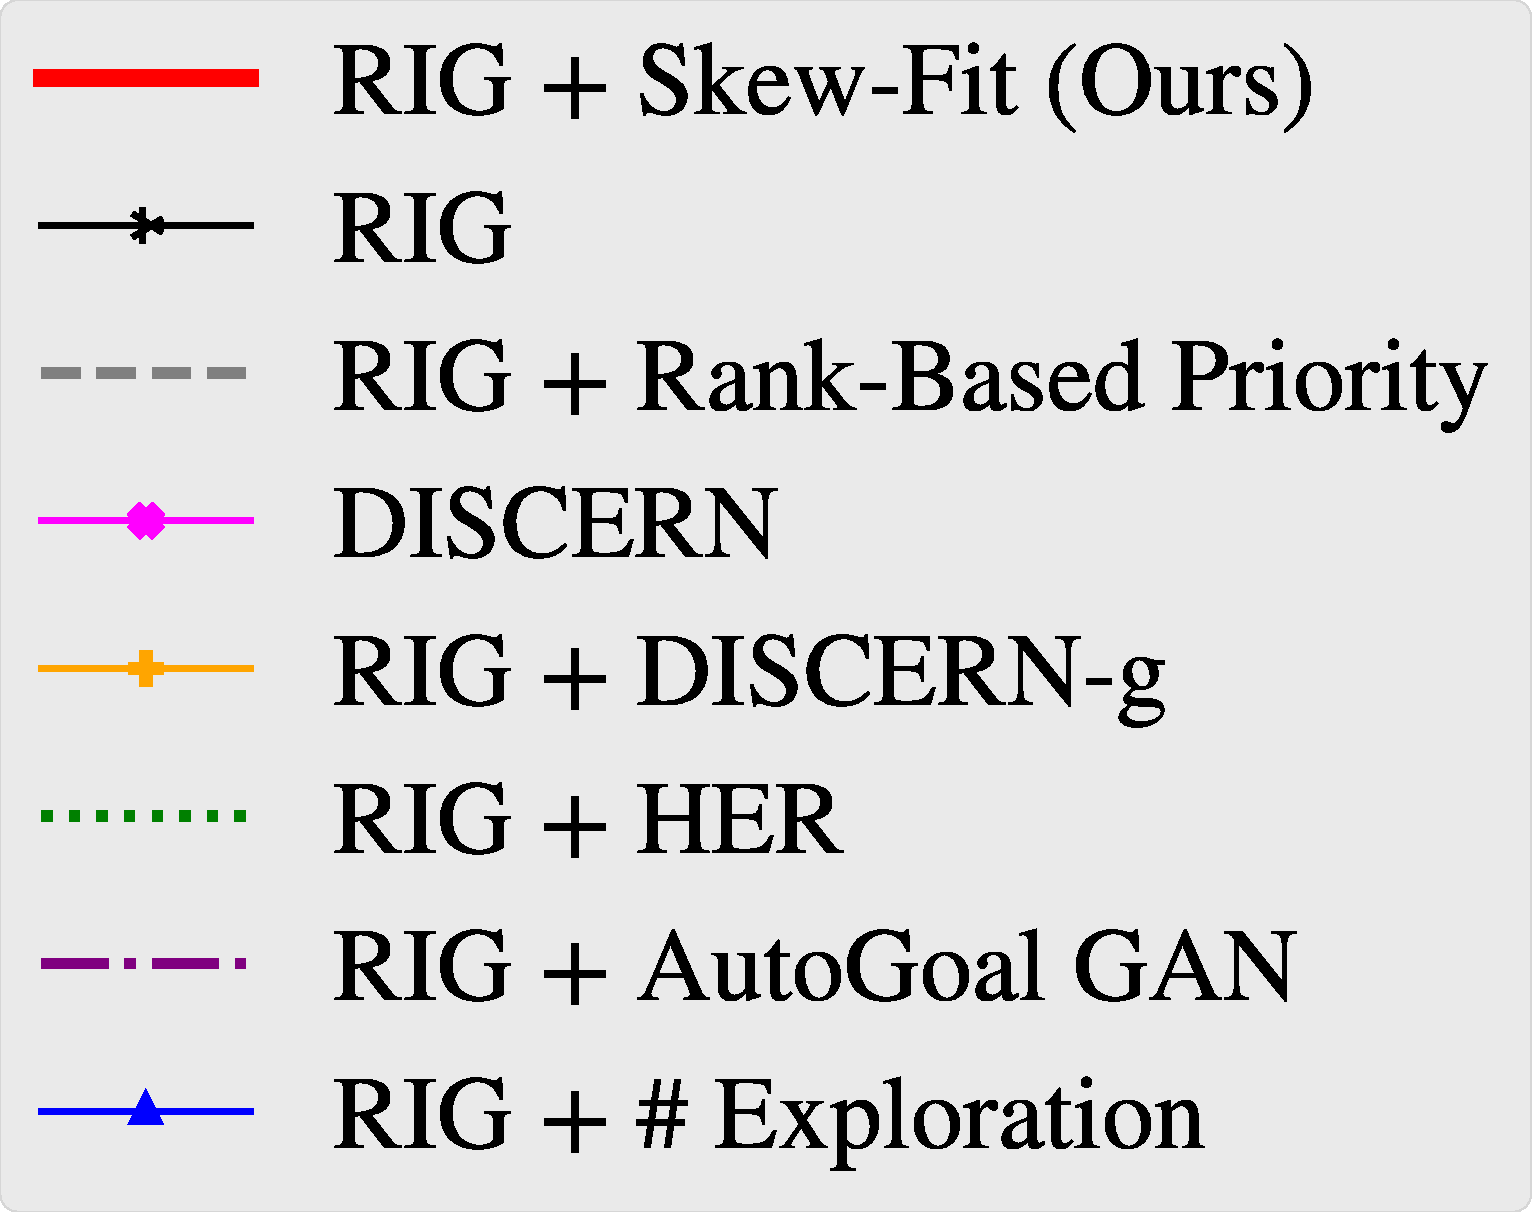
\includegraphics[width=0.8\linewidth]{skewfit/figures/plots/main_sim_fig/legend.pdf}
          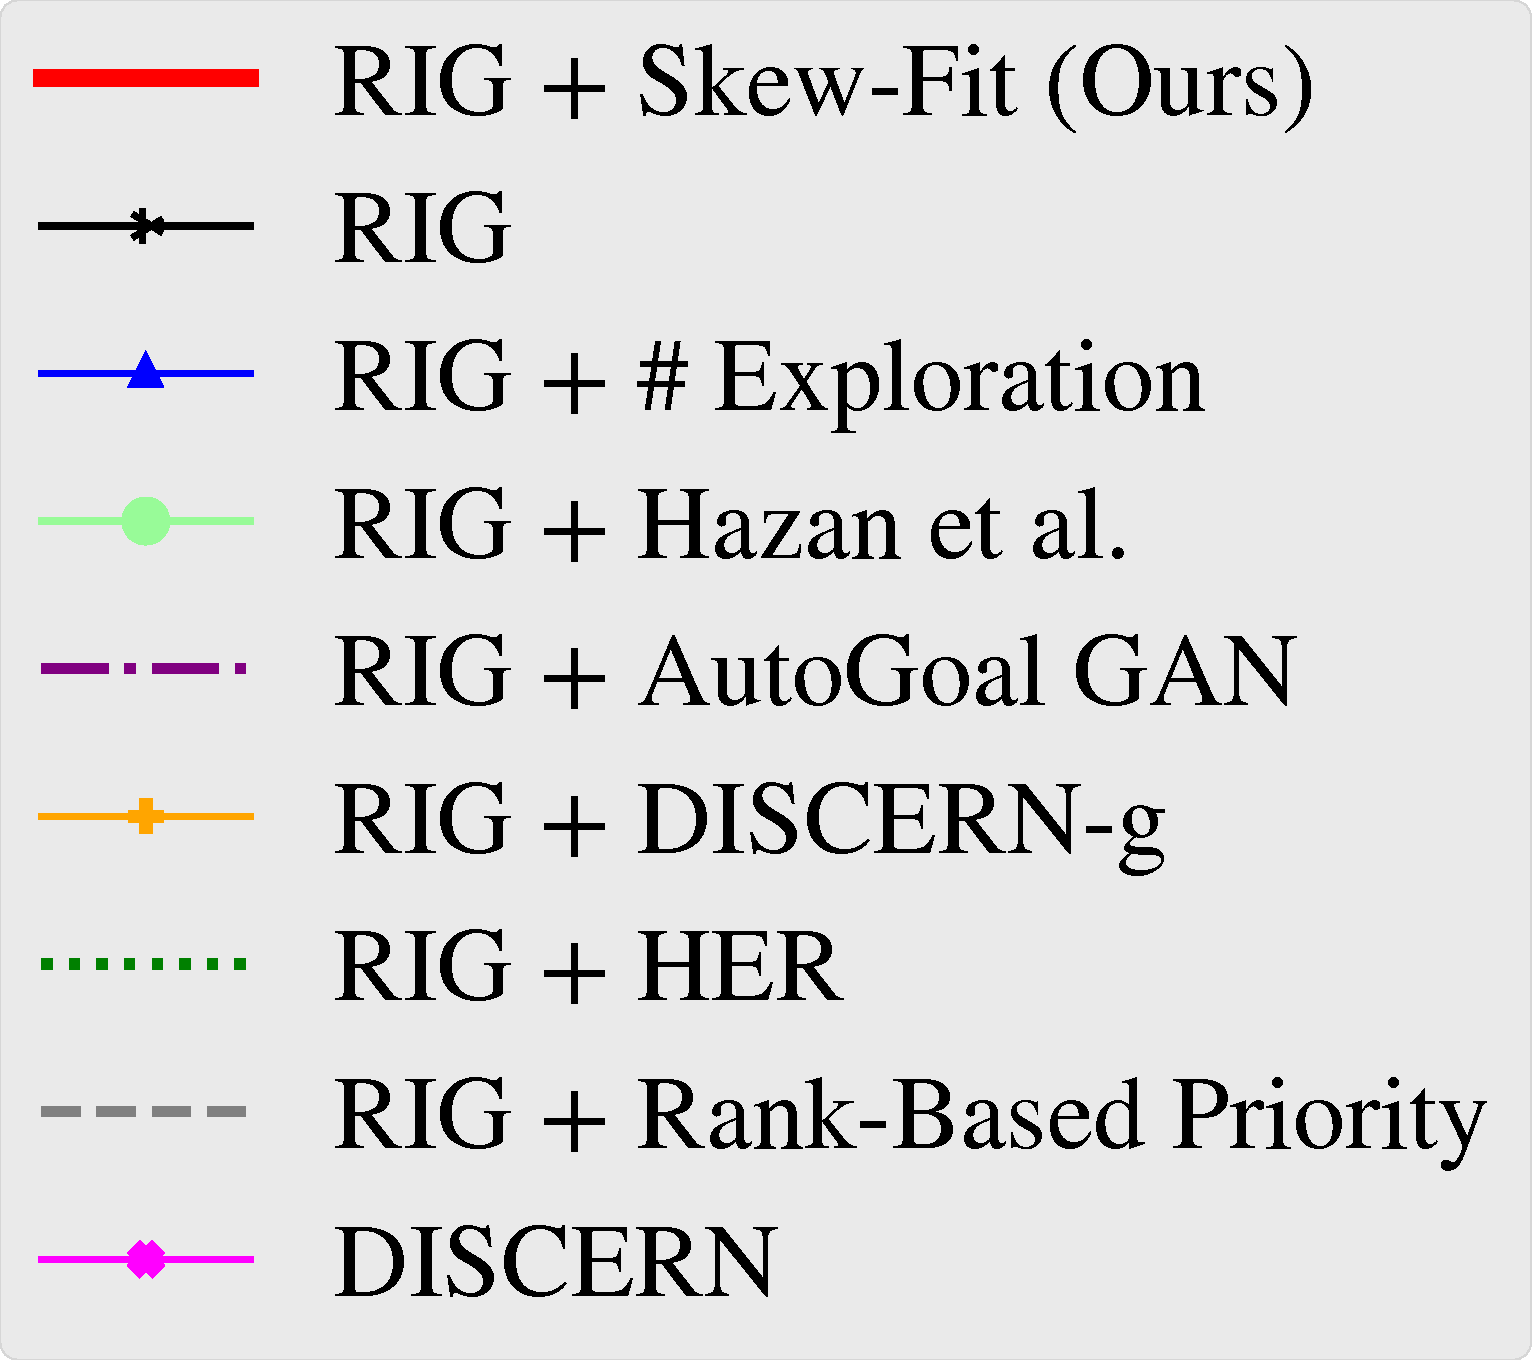
\includegraphics[width=\linewidth]{skewfit/figures/plots/main_sawyer_fig_with_hazan/main_figure_legend_with_hazan.pdf}
    }
  \end{subfigure}
    \fcaption{
        Learning curves for simulated continuous control tasks.
        Lower is better.
        We show the mean and standard deviation of 6 seeds and smooth temporally across 50 epochs within each seed.
        \METHOD consistently outperforms RIG and various prior methods.
        See text for description of each method.
    }
    \label{fig:sim-results}
\end{figure}


We see in \Figref{fig:sim-results} that Skew-Fit significantly outperforms prior methods both in terms of task performance and sample complexity.
The most common failure mode for prior methods is that the goal distributions collapse, resulting in the agent learning to reach only a fraction of the state space, as shown in \autoref{fig:offline-sk-real}.
For comparison, additional samples of $\pg$ when trained with and without \METHOD are shown in \autoref{sec:vae-dump}.
Those images show that without \METHOD, $\pg$ produces a small, non-diverse distribution for each environment: the object is in the same place for pickup, the puck is often in the starting position for pushing, and the door is always closed.
In contrast, \METHOD proposes goals where the object is in the air and on the ground, where the puck positions are varied, and the door angle changes.

We can see the effect of these goal choices by visualizing more example rollouts for RIG and \METHOD.
These visuals, shown in \Figref{fig:example_rollouts} in \autoref{sec:vae-dump}, show that RIG only learns to reach states close to the initial position, while \METHOD learns to reach the entire state space.
For a quantitative comparison, \Figref{fig:exploration_pickups} shows the cumulative total exploration pickups for each method.
From the graph, we see that many methods have a near-constant rate of object lifts throughout all of training.
\METHOD is the only method that significantly increases the rate at which the policy picks up the object during exploration, suggesting that only \METHOD sets goals that encourage the policy to interact with the object.

\begin{figure}[t]
\centering
  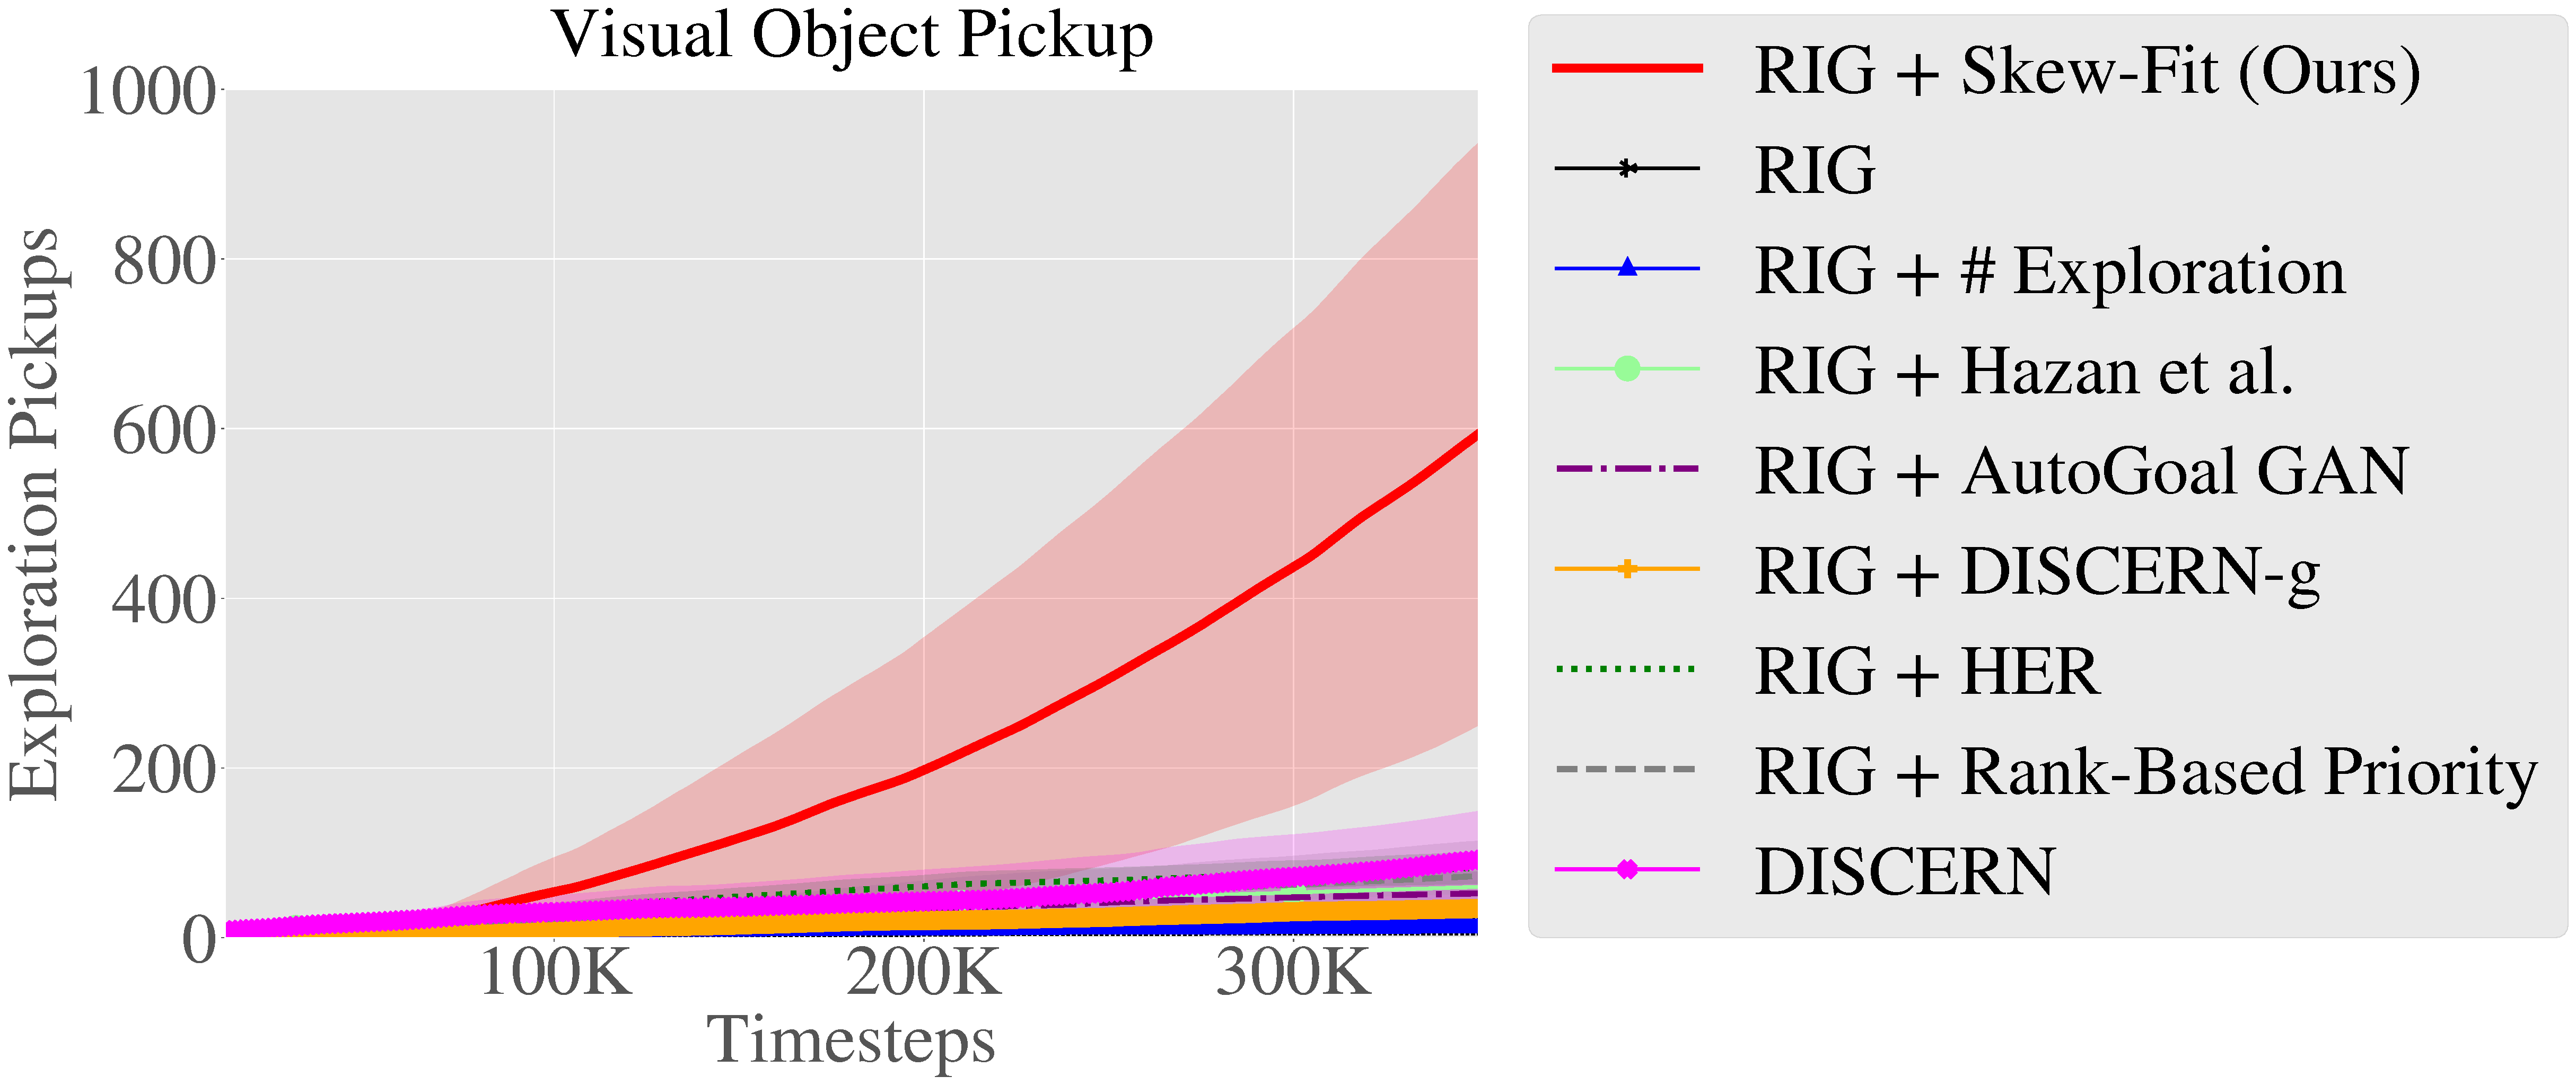
\includegraphics[width=\linewidth]{skewfit/figures/plots/exploration_pickups.pdf}
  \caption{
Cumulative total pickups during exploration for each method.
Prior methods fail to pay attention to the object: the rate of pickups hardly increases past the first 100 thousand timesteps.
In contrast, after seeing the object picked up a few times, \METHOD practices picking up the object more often by sampling the appropriate exploration goals.
}
  \label{fig:exploration_pickups}
\end{figure}


\paragraph{Real-World Vision-Based Robotic Manipulation}
We also demonstrate that \METHOD scales well to the real world with a door opening task, \textit{Real World Visual Door}, as shown in \Figref{fig:env-pics}.
While a number of prior works have studied RL-based learning of door opening~\cite{kalakrishnan2011learning,chebotar2017path}, we demonstrate the first method for autonomous learning of door opening without a user-provided, task-specific reward function.
As in simulation, we do not provide any goals to the agent and simply let it interact with the door, without any human guidance or reward signal.
We train two agents using RIG and RIG with \METHOD.
Every seven and a half minutes of interaction time, we evaluate on $5$ goals and plot the cumulative successes for each method.
Unlike in simulation, we cannot easily measure the difference between the policy's achieved and desired door angle.
Instead, we visually denote a binary success/failure for each goal based on whether the last state in the trajectory achieves the target angle.
As \Figref{fig:real-results} shows, standard RIG only starts to open the door after five hours of training.
In contrast, \METHOD learns to occasionally open the door after three hours of training and achieves a near-perfect success rate after five and a half hours of interaction.
\autoref{fig:real-results} also shows examples of successful trajectories from the \METHOD policy, where we see that the policy can reach a variety of user-specified goals.
These results demonstrate that \METHOD is a promising technique for solving real world tasks without any human-provided reward function.
Videos of \METHOD solving this task and the simulated tasks can be viewed on
our website.
\footnote{https://sites.google.com/view/skew-fit}

\begin{figure}[t]
  \centering
  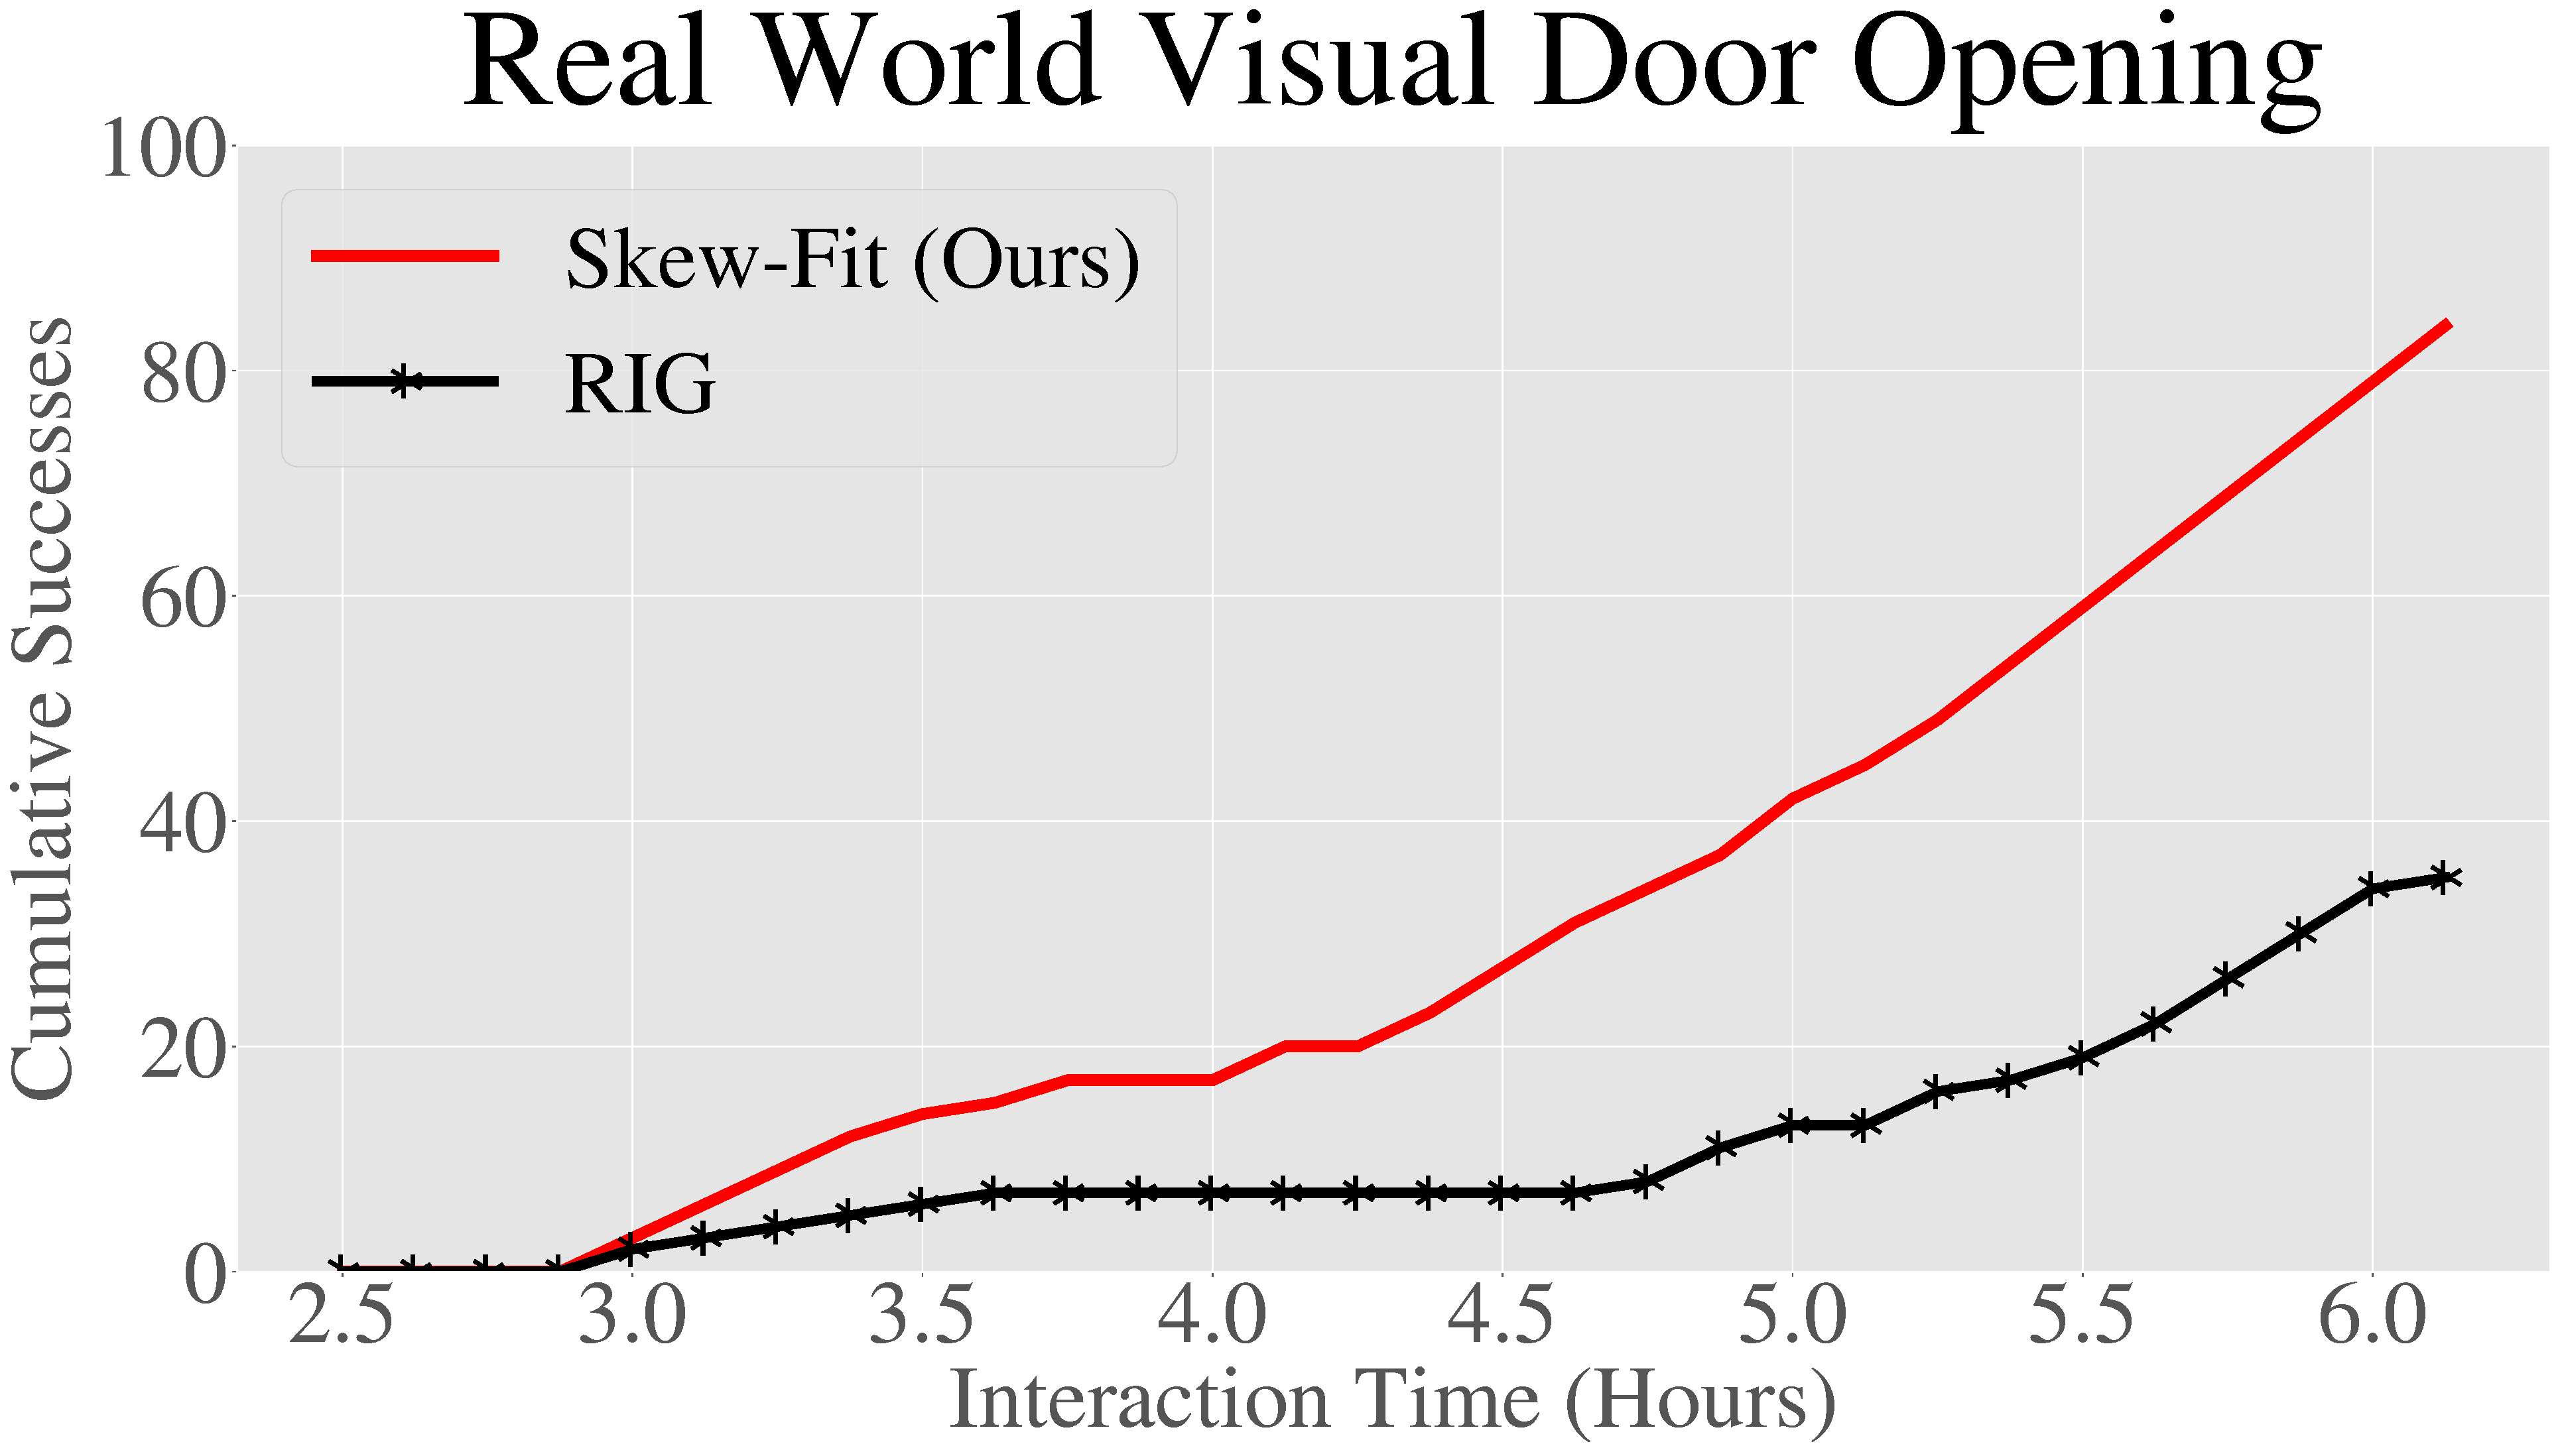
\includegraphics[width=0.75\linewidth]{skewfit/figures/plots/real_world_door.pdf}
    \begin{subfigure}[b]{0.49\textwidth}
        \center
        \hspace{-.2cm}
        $\SF_1$ \hspace{4.3cm} $\SF_{100}$ \hspace{.7cm} $\G$

        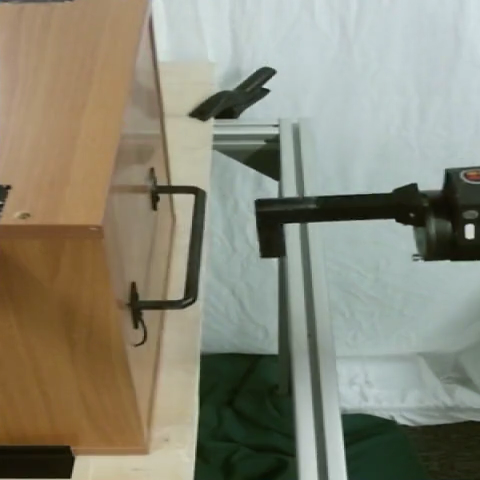
\includegraphics[width=0.14\linewidth]{skewfit/figures/imgs/real_env_rollout_new/door_easy/barely_open_5.png}
        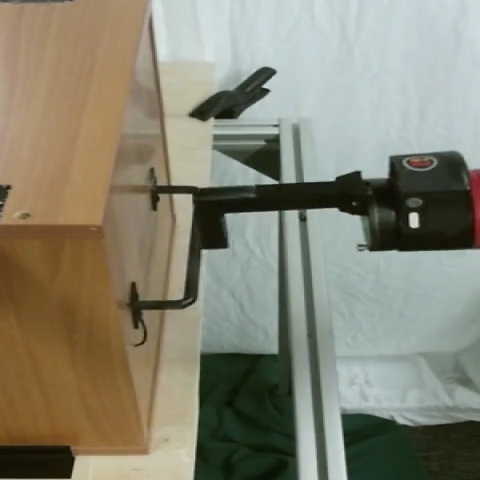
\includegraphics[width=0.14\linewidth]{skewfit/figures/imgs/real_env_rollout_new/door_easy/barely_open_10.png}
        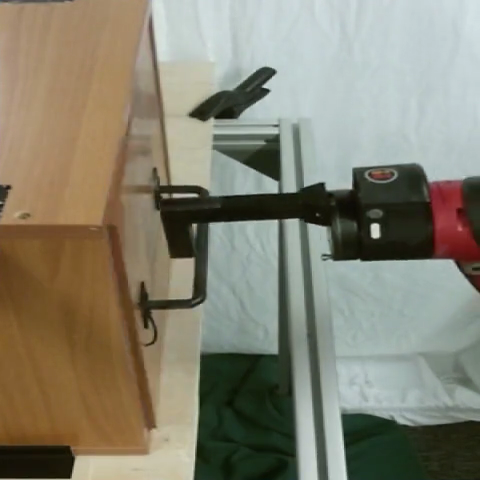
\includegraphics[width=0.14\linewidth]{skewfit/figures/imgs/real_env_rollout_new/door_easy/barely_open_15.png}
        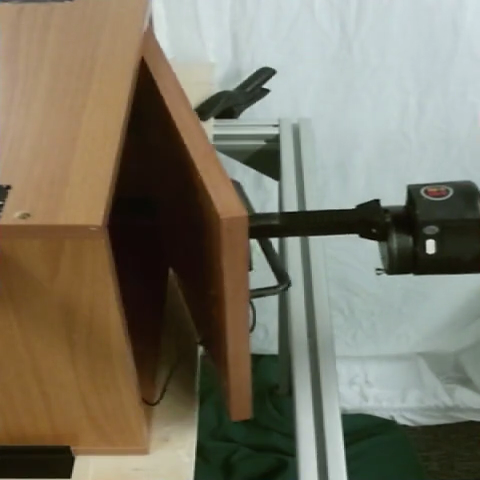
\includegraphics[width=0.14\linewidth]{skewfit/figures/imgs/real_env_rollout_new/door_easy/barely_open_20.png}
        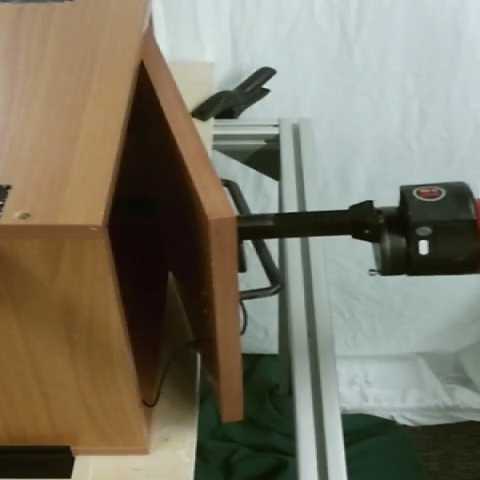
\includegraphics[width=0.14\linewidth]{skewfit/figures/imgs/real_env_rollout_new/door_easy/barely_open_25.png}
        \hspace{0.01\linewidth}
        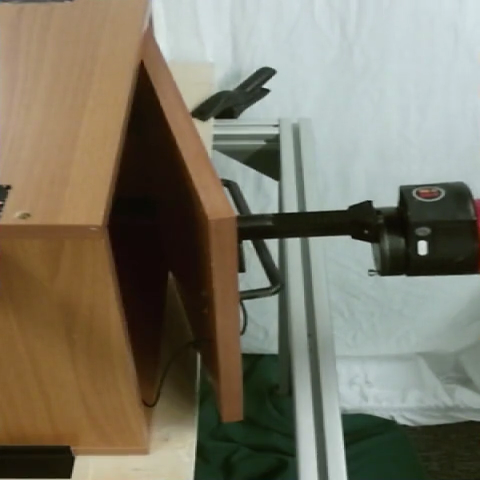
\includegraphics[width=0.14\linewidth]{skewfit/figures/imgs/real_env_rollout_new/door_easy/barely_open_45.png} %goal
    \end{subfigure}
    \begin{subfigure}[b]{0.49\textwidth}
        \center

        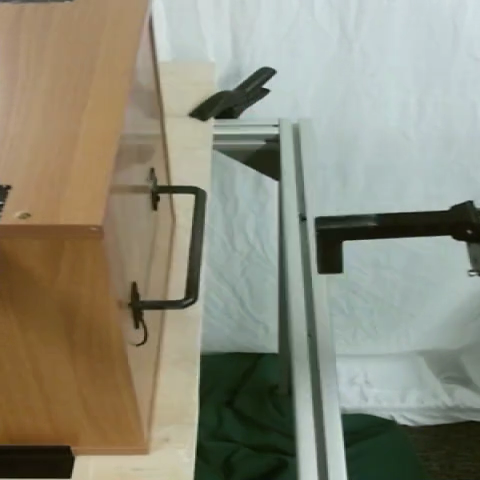
\includegraphics[width=0.14\linewidth]{skewfit/figures/imgs/real_env_rollout_novel/door_hard/wide_open_0.png}
        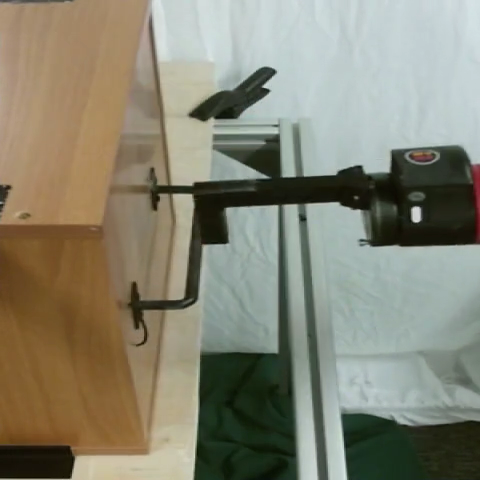
\includegraphics[width=0.14\linewidth]{skewfit/figures/imgs/real_env_rollout_novel/door_hard/wide_open_10.png}
        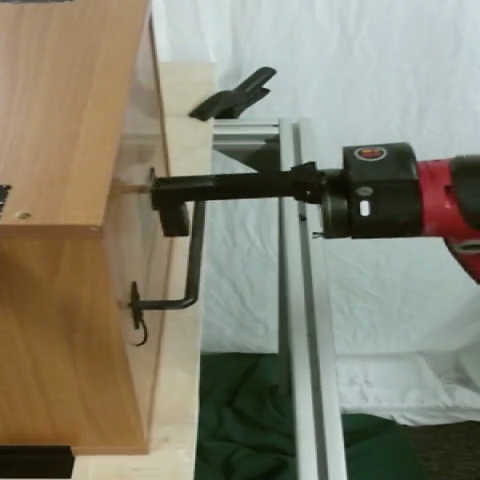
\includegraphics[width=0.14\linewidth]{skewfit/figures/imgs/real_env_rollout_novel/door_hard/wide_open_20.png}
        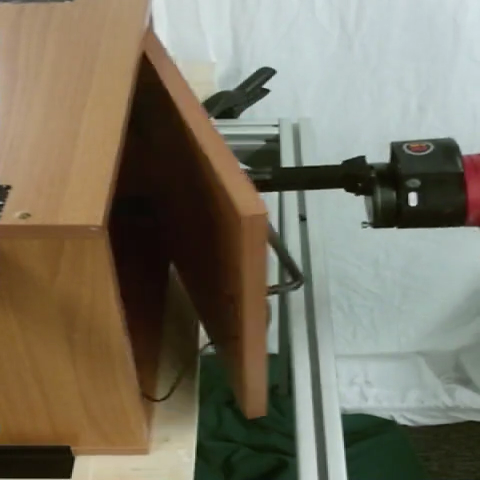
\includegraphics[width=0.14\linewidth]{skewfit/figures/imgs/real_env_rollout_novel/door_hard/wide_open_25.png}
        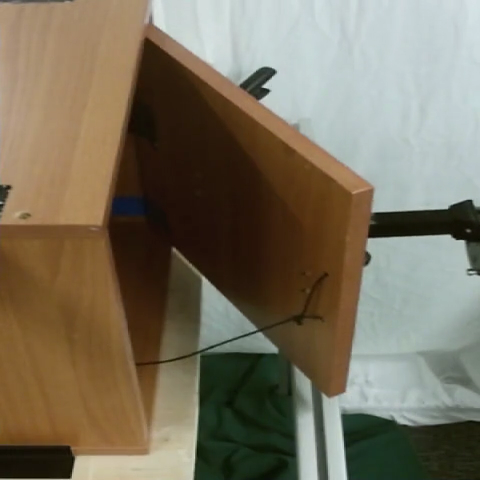
\includegraphics[width=0.14\linewidth]{skewfit/figures/imgs/real_env_rollout_novel/door_hard/wide_open_40.png}
        \hspace{0.01\linewidth}
        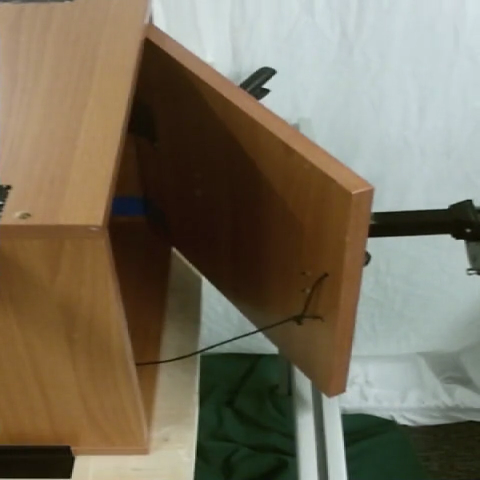
\includegraphics[width=0.14\linewidth]{skewfit/figures/imgs/real_env_rollout_novel/door_hard/wide_open_100.png}
    \end{subfigure}
  \fcaption{
  (Top) Learning curve for Real World Visual Door.
  \METHOD results in considerable sample efficiency gains over RIG on this real-world task.
  (Bottom)
  Each row shows the \METHOD policy starting from state $\SF_1$ and reaching state $\SF_{100}$ while pursuing goal $\G$.
  Despite being trained from only images without any user-provided goals during training, the \METHOD policy achieves the goal image provided at test-time, successfully opening the door.
  }
  \label{fig:real-results}
\end{figure}



\paragraph{Additional Experiments}
To study the sensitivity of \METHOD to the hyperparameter $\alpha$, we sweep $\alpha$ across the values $[-1, -0.75, -0.5, -0.25, 0]$ on the simulated image-based tasks.
The results are in \autoref{sec:add-exps} and demonstrate that \METHOD works across a large range of values for $\alpha$, and $\alpha=-1$ consistently outperform $\alpha=0$ (i.e. outperforms no \METHOD).
Additionally, \autoref{sec:implementation-details} provides a complete description our method hyperparameters, including network architecture and RL algorithm hyperparameters.